\section{The partial resolution and Gross's base}\label{sec:base}

This section constructs the two objects on which the rest of the paper works: the crepant partial resolution
$X'_\sigma$, with the lattice $K$ of relations among its exceptional curves, and Gross's integral affine base
$B=B'_\sigma$, with its discriminant $\Gamma$. It proves the properties of both that later sections use.

Proposition~\ref{prop:partialres} shows that $X'_\sigma$ has one ordinary double point for each node parallelogram,
and that in every small resolution the class of the exceptional curve $C_q$ is determined by its intersection numbers
with the divisors $D_r$, $r\in R$, which are the entries of the circuit $\circv_q$; so the rational relations among the
$[C_q]$ are exactly $K$. The proof compares an arbitrary small resolution with a maximal projective crepant partial
resolution of $X$ and does not use~\ref{hyp:P}. Proposition~\ref{prop:integral} shows that $H_2(\widehat X;\Z)$ is
torsion-free and detected by the $D_r$, so the integral relations are exactly $K$ as well; its proof combines a
Lefschetz theorem for the affine part of $X$ (Lemma~\ref{lem:lefschetz}) with a lattice property of admissible
polytopes (Lemma~\ref{lem:triple}) and duality. Proposition~\ref{prop:classical} describes the curves $C_q$ inside
the exceptional del Pezzo surface over a pentagon, an $A_1$ hexagon and an $A_2$ hexagon, and Remark~\ref{rem:tie}
records the resulting linear conditions (\emph{ties}) on the coordinates of $K$. On the base,
Proposition~\ref{prop:base} shows that $\Gamma$ is a graph whose four-valent vertices are negative nodes in the sense
of Casta\~no-Bernard and Matessi, one for each node parallelogram; Lemma~\ref{lem:full} shows that $\Gamma$ is a full
subcomplex of the barycentric subdivision of Gross's decomposition, and Lemma~\ref{lem:dualarc} describes $\Gamma$ inside the two-face of a
pentagon or hexagon. Proposition~\ref{prop:pulling} constructs the subdivision $\mathcal F_C$ of $\partial\Delta$ used on
the mirror side and proves that it satisfies a height condition at every node parallelogram. The proof rests on a
count of lattice points in a pyramid over a unit parallelogram (Lemma~\ref{lem:pyramid}). Section~\ref{ssec:proj}
identifies~\ref{hyp:P} with the projectivity of $X'_\sigma\to X$ and describes an explicit obstruction to it.

Throughout, $\Delta$ is admissible (Definition~\ref{def:admissible}) and $\sigma$ is a profile
(Definition~\ref{def:profile}). Hypothesis~\ref{hyp:P} is assumed in Sections~\ref{ssec:gross}--\ref{ssec:mirrorsub},
and in Section~\ref{ssec:partialres} where stated; Section~\ref{ssec:proj} does not assume it. The pair
$(\mathcal T,\check h)$ is the one provided by Theorem~\ref{thm:U}.

\subsection{Admissible two-faces and profiles}\label{ssec:faces}
Let $G$ be a $dP_7$ pentagon or a $dP_6$ hexagon, with $k=5$ or $6$ vertices $w_0,\dots,w_{k-1}$ in cyclic order and
centre $o$; indices of the $w_j$ are taken modulo $k$. For each $j$ put
\[
T_j=\operatorname{conv}\{o,w_j,w_{j+1}\},\qquad P_j=\operatorname{conv}\{o,w_j,w_{j+1},w_{j+2}\}.
\]
Up to $GL_2(\Z)$ and translation there is exactly one lattice pentagon and exactly one lattice hexagon with one
interior lattice point and no boundary lattice points other than their vertices, since the lattice polygons with
exactly one interior lattice point form sixteen classes \cite{PRV00}. The hexagon is the one of
Section~\ref{ssec:admissible}. The pentagon has, in suitable coordinates, the vertices
\begin{equation}\label{eq:pentnormal}
w_0,\dots,w_4=(1,0),\ (1,1),\ (0,1),\ (-1,0),\ (0,-1),\qquad o=(0,0).
\end{equation}

\begin{lemma}[subdivisions of the del Pezzo faces]\label{lem:subdiv}
\begin{enumerate}
\item Every triangle $T_j$ is unimodular, every segment $[o,w_j]$ is primitive, and $P_j$ is a unit parallelogram if and
only if $w_j+w_{j+2}=o+w_{j+1}$. For the hexagon this holds for every $j$; for the pentagon~\eqref{eq:pentnormal} it holds
exactly for $j\in\{4,0,1\}$.
\item The subdivisions of $G$ into unit parallelograms and unimodular triangles all of which contain $o$ are the
subdivisions into cells $T_j$ and $P_j$ whose edges at $o$ are consecutive segments $[o,w_j]$.
\item A pentagon has exactly one such subdivision with two parallelograms; in the coordinates~\eqref{eq:pentnormal} it
consists of $P_4$, $P_1$ and $T_3$. A hexagon has exactly three such subdivisions in which two parallelograms meet only
in $o$, namely $\{P_j,T_{j+2},P_{j+3},T_{j+5}\}$ for $j\in\{0,1,2\}$ (the $A_1$ subdivisions of
Definition~\ref{def:profile}), and exactly two with three parallelograms, namely $\{P_j:j\equiv j_0\bmod2\}$ for
$j_0\in\{0,1\}$ (the $A_2$ subdivisions).
\item Every cell of these subdivisions, and every face of such a cell, has no lattice points other than its vertices.
\end{enumerate}
\end{lemma}

\begin{proof}
(1) By Pick's formula $G$ has normalised area $2\cdot1+k-2=k$. It is the union of the $k$ triangles $T_j$, whose
normalised areas are positive integers; so each is $1$. An interior lattice point of $[o,w_j]$ would be a second interior
lattice point of $G$. If $w_j+w_{j+2}=o+w_{j+1}$, then $o,w_j,w_{j+1},w_{j+2}$ are the vertices of a parallelogram in this
cyclic order, the union of the unimodular triangles $T_j$ and $T_{j+1}$; conversely, in a parallelogram with vertices in
this cyclic order the sums of opposite vertices agree. For the hexagon the relation is stated in
Section~\ref{ssec:admissible}. For~\eqref{eq:pentnormal}, $w_4+w_1=w_0$, $w_0+w_2=w_1$ and $w_1+w_3=w_2$, while $w_2+w_4=0\ne
w_3$ and $w_3+w_0=0\neq w_4$.

(2) Unit parallelograms and unimodular triangles contain no lattice points besides their vertices, so $o$ is a vertex of
every cell, and the other vertices are among the $w_j$. The edges of the subdivision at $o$ are segments $[o,w_j]$; they
cut $G$ into sectors, and a cell containing $o$ is the sector between two consecutive such edges $[o,w_j]$ and
$[o,w_{j+m}]$, because it contains the part of $\partial G$ between $w_j$ and $w_{j+m}$. That sector is
$\operatorname{conv}\{o,w_j,\dots,w_{j+m}\}$, a polygon with $m+2$ vertices. So $m=1$ and the cell is $T_j$, or $m=2$ and the
cell is $P_j$, which must then be a unit parallelogram.

(3) By (2) the subdivisions correspond to the ways of cutting the cyclic sequence of the $k$ boundary edges of $G$ into
runs of length $1$ (a triangle) and $2$ (a parallelogram $P_j$, allowed only where the relation of (1) holds). For the
pentagon with two parallelograms the runs are $2,2,1$, starting at $j$, $j+2$ and $j+4$; by (1) both $j$ and $j+2$ must
lie in $\{4,0,1\}$, which forces $j=4$. For the hexagon every run of length $2$ is allowed. Two parallelograms meeting
only in $o$ are separated on both sides by a triangle, so the runs are $2,1,2,1$ starting at $j,j+2,j+3,j+5$, and $j$ is
determined modulo $3$. Three parallelograms fill the hexagon with runs $2,2,2$, determined by the parity of $j$.

(4) This holds for unimodular triangles, unit parallelograms, the edges of $G$, which are primitive by admissibility,
and the segments $[o,w_j]$, which are primitive by (1).
\end{proof}

The remaining subdivisions of the hexagon in (2), with no parallelogram, with one, or with two parallelograms sharing an
edge, do not occur in profiles. Up to rotation, the $A_1$ and $A_2$ subdivisions are the local models $W_{6,1}$ and $W_{6,2}$ of
\cite[Prop.~3.7(2),(3)]{Paper5}. The pentagon subdivision gives the two-node model described in
Section~\ref{ssec:partialres}.

By Lemma~\ref{lem:subdiv}(4) and admissibility, the lattice points of $\Delta$ on faces of dimension at most two are the
vertices of $\Delta$ and the centres of the pentagons and hexagons, which is the set $R$ of
Section~\ref{ssec:admissible}; each of them is a vertex of the subdivision that $\sigma$ induces on every two-face
containing it. For a two-face $G$ that is not a triangle we write $G^\circ=[u,u']$; since $\ell(G^\circ)=1$, $u$ and $u'$
are lattice points and vertices of $\Delta^\circ$, and the facets $u^\vee=\{n\in\Delta:\langle u,n\rangle=-1\}$ and
$u'^\vee$ of $\Delta$ satisfy $u^\vee\cap u'^\vee=G$. We write $N_G:=\{u,u'\}^\perp\cap N$ for the lattice of the plane of $G$. Put
\[
e_{u'}(n):=\langle u',n\rangle+1,\qquad e_u(n):=\langle u,n\rangle+1\qquad(n\in N).
\]
Both are nonnegative on $\Delta$; $e_{u'}$ vanishes on $u^\vee$ exactly along $G$.

\begin{lemma}[the dual edge]\label{lem:primheight}
Let $G$ be a two-face of $\Delta$ that is not a triangle, with $G^\circ=[u,u']$. Then $\Z u+\Z u'$ is a saturated
sublattice of $M$. Hence there is $w_{u'}\in N$ with $\langle u,w_{u'}\rangle=0$ and $\langle u',w_{u'}\rangle=1$, and
$u^\perp\cap N=N_G\oplus\Z w_{u'}$. In particular $e_{u'}$ is a primitive
affine function on the lattice of $\operatorname{aff}(u^\vee)$.
\end{lemma}

\begin{proof}
Let $L=(\R u+\R u')\cap M$, a saturated sublattice of rank two. Since $\ell(G^\circ)=1$, $u'-u$ is primitive in $M$, hence
in $L$; complete it to a basis $(u'-u,f)$ of $L$ and write $u=x(u'-u)+yf$ with $x,y\in\Z$. For a vertex $a$ of $G$,
$\langle u,a\rangle=\langle u',a\rangle=-1$, so $\langle u'-u,a\rangle=0$ and $-1=y\langle f,a\rangle$; hence $y=\pm1$, and
$(u'-u,u)$ is a basis of $L$. So $L=\Z u+\Z u'$. A saturated sublattice spanned by $u,u'$ extends to a basis of $M$, and the
dual basis contains a vector $w_{u'}$ as stated. For $n\in u^\perp\cap N$ the vector $n-\langle u',n\rangle w_{u'}$ lies in $N_G$.
\end{proof}

The vectors $w_{u'}$ (and $w_u$, with $u$ and $u'$ exchanged) are the ones used at the node points in Section~\ref{ssec:member}. The lemma uses only reflexivity and $\ell(G^\circ)=1$. The lattice point $a$ on the level $-1$ of both $u$ and $u'$ is
needed: $u=(1,0)$ and $u'=(2,2)$ have primitive difference and span a sublattice of index two.

\subsection{The partial resolution, the small resolution and \texorpdfstring{$K$}{K}}\label{ssec:partialres}
\emph{The singular points of $X$.} For a two-face $G$ of $\Delta$ let $\tau_G=\operatorname{cone}(G)$. Since $G$ lies in
the hyperplane $\{\langle u,\cdot\rangle=-1\}$, the affine toric variety of $\tau_G$ is $U_G\times\C^*$, where $U_G$ is the
three-dimensional Gorenstein affine toric variety of $\tau_G$ in the lattice $N\cap\operatorname{span}(G)$: the cone over
the toric surface of the polygon $G$, embedded by its anticanonical class. The orbit $O(\tau_G)\cong\C^*$ is the curve
$\{0\}\times\C^*$. As $X$ is $\Delta^\circ$-regular, it meets $O(\tau_G)$ transversally in $\ell(G^\circ)=1$ point $x_G$
\cite[\S3]{Batyrev}: the equation of $X$ restricted to the orbit is a Laurent polynomial in one variable with a simple
zero. By the implicit function theorem, near $x_G$ the hypersurface $X$ is the graph of a holomorphic function
$U_G\to\C^*$, so the projection to $U_G$ identifies a neighbourhood of $x_G$ in $X$ with a neighbourhood of the vertex of
$U_G$. Thus $x_G$ is a node when $G$ is a unit square, a cone over $dP_7$ when $G$ is a pentagon, and a cone over $dP_6$
when $G$ is a hexagon. The cones over the edges and the unimodular triangles of $\Delta$ are generated by parts of lattice
bases, so $\mathbb P_\Delta$ is smooth along their orbits and so is $X$; and $X$ misses the torus-fixed points of
$\mathbb P_\Delta$, since its equation restricted to such a point is the coefficient of a vertex of $\Delta^\circ$, which
is nonzero. So the singular points of $X$ are the points $x_G$, one for each square, pentagon and hexagon.

\emph{The partial resolution.} The profile $\sigma$ subdivides $\tau_G$ into the cones over its cells; let
$U'_{G,\sigma}\to U_G$ be the corresponding toric morphism. The \emph{partial resolution} $X'_\sigma\to X$ replaces a
neighbourhood of each $x_G$ by the corresponding neighbourhood of the fibre over the vertex in $U'_{G,\sigma}$, and is an
isomorphism elsewhere; since the $x_G$ are isolated, this defines a compact complex space. Under~\ref{hyp:P} it is the
proper transform of $X$ in $P'_\sigma$ of Section~\ref{ssec:admissible}: the cones of the fan of $P'_\sigma$ in the cone
over a face of dimension at most two are the cones over the cells of $\sigma$, and $X$ meets no orbit of a cone that is
not contained in such a cone. Similarly, a \emph{small resolution} $\widehat X\to X'_\sigma$ is locally, at each node,
one of the two small resolutions of the cone $\{xy=zw\}$. At the node of the parallelogram $abcd$ they are the toric
resolutions given by the triangles $abc,acd$ (the diagonal $\{a,c\}$) or $abd,bcd$ (the diagonal $\{b,d\}$). So near the
preimage of $x_G$, a small resolution is the toric resolution of $U_G$ given by the triangulation of $G$ obtained from
$\sigma$ by one diagonal in each parallelogram. Every small resolution is a compact complex manifold with trivial
canonical class, since $X'_\sigma\to X$ and $\widehat X\to X'_\sigma$ are crepant and $K_X=0$ \cite[\S4]{Batyrev}.

\emph{The divisors $D_r$.} For a vertex $r$ of $\Delta$ let $D_r\subset\widehat X$ be the proper transform of the surface
$X\cap D^\Delta_r$, where $D^\Delta_r$ is the toric divisor of $\mathbb P_\Delta$ of the ray through $r$; for the centre $o$
of a pentagon or hexagon $G$ let $D_o\subset\widehat X$ be the exceptional surface over $x_G$. Near the preimage of $x_G$,
$D_r$ is the toric divisor of the ray through $r$ in the local model, for every $r\in R\cap G$. As $\widehat X$ is smooth,
each $D_r$ is a Cartier divisor, with a class $D_r\in H^2(\widehat X;\Z)$. When $\widehat X$ is the proper transform of $X$
in a toric variety refining the fan of $\mathbb P_\Delta$, $D_r$ is the restriction of the toric divisor of the ray through
$r$; toric divisors of rays not through points of $R$ restrict to zero, because their orbits lie over torus-fixed points
of $\mathbb P_\Delta$.

\begin{lemma}\label{lem:H2}
For every small resolution $\widehat X$ of $X'_\sigma$ the classes $D_r$, $r\in R$, span $H^2(\widehat X;\Q)$. Hence
\begin{equation}\label{eq:injection}
H_2(\widehat X;\Q)\longrightarrow\Q^R,\qquad C\longmapsto(D_r\cdot C)_{r\in R},
\end{equation}
is injective. This does not require~\ref{hyp:P}.
\end{lemma}

\begin{proof}
Let $\mathcal S_0$ be a regular fine triangulation of $\partial\Delta$, that is, one whose vertices are all the lattice
points of $\partial\Delta$, let $P_0$ be the projective toric variety of the fan over it, and let $\widehat X_0$ be the
proper transform of $X$ in $P_0$. It is a maximal projective crepant partial resolution in the sense of Batyrev, and a
smooth threefold. By \cite[Prop.~8.3]{Paper4} the restrictions of the toric divisors of $P_0$ span $H^2(\widehat X_0;\Q)$.
That proposition applies because every two-face of $\Delta$ is a unimodular triangle or has a dual edge of lattice length
one, so that the correction term in Batyrev's formula for $h^{1,1}$ vanishes. The toric divisors of rays outside $R$
restrict to zero, so the $D_r$, $r\in R$, span $H^2(\widehat X_0;\Q)$.

Near the preimage of each singular point $x_G$, both $\widehat X$ and $\widehat X_0$ are toric resolutions of $U_G$ given by
triangulations of $G$ with the same vertex set, the lattice points of $G$. Both fans contain the subfan consisting of the
rays and of the cones over the edges of $G$, so both toric varieties contain its toric variety as an open subset. The
complements are the orbits of the cones that meet the interior of $\tau_G$ in dimension two or three; these lie over the
vertex of $U_G$ and are compact curves and points. Hence there are compact unions of curves
$Z\subset\widehat X$ and $Z_0\subset\widehat X_0$, lying over the points $x_G$, and an isomorphism
$\widehat X\setminus Z\cong\widehat X_0\setminus Z_0=:U$, compatible with the maps to $X$, that carries $D_r\cap(\widehat X\setminus Z)$
to $D_r\cap U$ for every $r\in R$. The set $Z$ is a compact analytic subset of the compact complex manifold $\widehat X$,
hence a subcomplex of a triangulation of $\widehat X$ \cite[Thm.~2]{Loj64} and locally contractible. The duality
$H_i(M,M\setminus K;\Z)\cong H^{n-i}(K;\Z)$ for a compact, locally contractible subset $K$ of a closed oriented
$n$-manifold $M$ \cite[Thm.~3.44]{Hat02} gives $H_k(\widehat X,\widehat X\setminus Z;\Z)\cong H^{6-k}(Z;\Z)$, which
vanishes for $k\le3$ because $Z$ is a polyhedron of dimension at most two. By universal coefficients over the field $\Q$,
$H^k(\widehat X,\widehat X\setminus Z;\Q)\cong\operatorname{Hom}(H_k(\widehat X,\widehat X\setminus Z;\Z),\Q)=0$ for $k\le3$.
The exact sequence of the pair gives
\begin{equation}\label{eq:H2restr}
H^2(\widehat X;\Q)\xrightarrow{\ \cong\ }H^2(U;\Q),
\end{equation}
and likewise $H^2(\widehat X_0;\Q)\cong H^2(U;\Q)$. The two isomorphisms carry $D_r$ to the class of $D_r\cap U$. So the
$D_r$, $r\in R$, span $H^2(\widehat X;\Q)$, and~\eqref{eq:injection} is injective because the evaluation pairing
$H_2(\widehat X;\Q)\times H^2(\widehat X;\Q)\to\Q$ is perfect.
\end{proof}

\begin{proposition}\label{prop:partialres}
Let $\Delta$ be admissible and $\sigma$ a profile.
\begin{enumerate}
\item $X'_\sigma$ has exactly one singular point for each node parallelogram, an ordinary double point, and is smooth
elsewhere. Under~\ref{hyp:P}, $X'_\sigma\to X$ is induced by the projective toric morphism $P'_\sigma\to\mathbb P_\Delta$.
\item Let $\widehat X$ be a small resolution of $X'_\sigma$. If $\widehat X$ uses the diagonal $\{a,c\}$ at the node $q$ of the
parallelogram $abcd$, the image of $[C_q]$ under~\eqref{eq:injection} is $\circv_q=e_b+e_d-e_a-e_c$; if it uses $\{b,d\}$,
it is $-\circv_q$. Consequently, for the small resolution with the chosen diagonals,
\[
\Bigl\{\lambda\in\Z^Q:\ \sum_q\lambda_q[C_q]=0\text{ in }H_2(\widehat X;\Q)\Bigr\}=K,
\]
and the classes $[C_q]$ span a subspace of $H_2(\widehat X;\Q)$ of dimension $|Q|-\operatorname{rank}K$. When $\widehat X$ is
projective, this is the relative Picard number of $\widehat X\to X'_\sigma$.
\item Assume~\ref{hyp:P}. The small resolution with the chosen diagonals is projective if and only if no nonzero
$\lambda\in K$ has all $\lambda_q\ge0$; it is then the proper transform of $X$ in the toric variety of a regular
refinement of $\Sigma'$. The diagonals at the squares can always be chosen so that this holds.
\end{enumerate}
\end{proposition}

\begin{proof}
(1) Let $P=abcd$ be a node parallelogram in the two-face $G$. The cone over $P$ is generated by four vectors with
$a+c=b+d$ that span a saturated sublattice of rank three, so its affine toric variety is $\{xy=zw\}\times\C^*$. In the local
model $U'_{G,\sigma}$ over $x_G$ it contributes the torus-fixed point of the cone over $P$, an ordinary double point; the
other cells of $\sigma|_G$ are unimodular triangles and primitive segments (Lemma~\ref{lem:subdiv}(4)), whose cones are
smooth. Over the squares, $X'_\sigma=X$ near $x_G$, which is a node. The other points of $X'_\sigma$ lie over smooth points of
$X$. The second sentence was shown above.

(2) Near $C_q$, $\widehat X$ is the small resolution of the cone $\{xy=zw\}$ given by the three-dimensional cones
$\operatorname{cone}(a,b,c)$ and $\operatorname{cone}(a,c,d)$, and $C_q$ is the curve of their common wall
$\operatorname{cone}(a,c)$. The divisors $D_a,\dots,D_d$ are there the toric divisors of the local model, and the wall
relation $b+d-a-c=0$ gives $D_b\cdot C_q=D_d\cdot C_q=1$ and $D_a\cdot C_q=D_c\cdot C_q=-1$. A divisor $D_r$ with
$r\notin\{a,b,c,d\}$ is disjoint from $C_q$, because in the local model the orbit closure of the ray through $r$ contains
the orbit of $\operatorname{cone}(a,c)$ only if $r\in\{a,c\}$, and the other orbits of $\widehat X$ over $x_G$ that meet
$C_q$ are those of $\operatorname{cone}(a,b,c)$ and $\operatorname{cone}(a,c,d)$. Hence $[C_q]\mapsto\circv_q$, and the
other diagonal exchanges the roles of $\{a,c\}$ and $\{b,d\}$. Since~\eqref{eq:injection} is injective
(Lemma~\ref{lem:H2}), $\sum_q\lambda_q[C_q]=0$ if and only if $\sum_q\lambda_q\circv_q=0$, and the span of the $[C_q]$ is
isomorphic to that of the $\circv_q$, of dimension $|Q|-\operatorname{rank}K$. When $\widehat X$ is projective, the divisors $D_r$
span $H^2(\widehat X;\Q)$ (Lemma~\ref{lem:H2}), so a rational combination of curves is numerically trivial if and only if its class in
$H_2(\widehat X;\Q)$ vanishes; hence the span of the contracted curves in $N_1(\widehat X/X'_\sigma)\otimes\Q$ has the same
dimension.

(3) If an ample class $L$ exists on $\widehat X$, then $L\cdot C_q>0$ for all $q$, and a relation
$\sum_q\lambda_q[C_q]=0$ with $\lambda\ge0$ forces $\lambda=0$. Conversely, suppose no nonzero $\lambda\ge0$ lies in $K$. By
Gordan's alternative there is $\psi\in\Q^R$ with $\langle\circv_q,\psi\rangle>0$ for every $q$; extend $\psi$ by $0$ to the
other lattice points of $\partial\Delta$. Let $h$ be a strictly convex function inducing $\Sigma'$. For $\epsilon>0$ small,
the strict inequalities by which $h$ exceeds its linear piece on the cone over a cell of $\Sigma'$ at the lattice points
outside that cell persist for $h+\epsilon\psi$, so the subdivision it induces refines $\Sigma'$ and subdivides each cell
$\omega$ of $\Sigma'$ by the regular subdivision of $\omega\cap N$ induced by $\psi|_\omega$. This subdivision may use
lattice points of $\omega$ that are not vertices of $\omega$; these lie in the relative interiors of facets of $\Delta$,
and the proper transform of $X$ meets no orbit of a cone containing one of them, since such an orbit lies over a
torus-fixed point of $\mathbb P_\Delta$. A unimodular triangle or a primitive segment is not subdivided, and $\psi$ subdivides a parallelogram $abcd$ by the diagonal
$\{a,c\}$ if and only if $\psi(a)+\psi(c)<\psi(b)+\psi(d)$, that is, $\langle\circv_q,\psi\rangle>0$. The toric variety of
the refined fan is projective, it is smooth along the orbits that $X$ meets, and the proper transform of $X$ in it is the
small resolution with the chosen diagonals. For the last sentence take $\psi$ equal to $-1$ at the centres and to small
generic values at the vertices of $\Delta$, and choose at each square the diagonal $\{a,c\}$ with $\langle\circv_q,\psi\rangle>0$.
At a parallelogram of a pentagon or hexagon, whose chosen diagonal passes through the centre, $\langle\circv_q,\psi\rangle$ is
$1$ plus a small number.
\end{proof}

When every singular two-face is a unit square, the identification of the classes $[C_q]$ with the circuits is stated in
\cite[\S2]{BK10}. The relations hold integrally (Proposition~\ref{prop:integral} below).

\subsubsection*{Integral relations among the exceptional curves}

Proposition~\ref{prop:partialres}(2) determines the relations among the classes $[C_q]$ in rational homology. They
hold integrally, because $H_2(\widehat X;\Z)$ is torsion-free and is detected by the divisors $D_r$. Let $T=N\otimes\C^*$
be the dense torus of $\mathbb P_\Delta$ and $W=X\cap T$. The singular points $x_G$ of $X$ lie on orbits of cones over
two-faces, so $W$ lies in the locus over which $\widehat X\to X$ is an isomorphism, and we regard $W$ as an open subset
of $\widehat X$. It is the affine hypersurface in $T$ of a Laurent polynomial with Newton polytope $\Delta^\circ$.

\begin{proposition}[integral relations among the exceptional curves]\label{prop:integral}
Let $\Delta$ be admissible, $\sigma$ a profile and $\widehat X$ any small resolution of $X'_\sigma$, with the node
parallelograms labelled by the diagonals of $\widehat X$. Then:
\begin{enumerate}
\item the homomorphism
\begin{equation}\label{eq:iotaZ}
\mathrm{ev}_D\colon H_2(\widehat X;\Z)\longrightarrow\Z^R,\qquad C\longmapsto(D_r\cdot C)_{r\in R},
\end{equation}
is injective; in particular $H_2(\widehat X;\Z)$ is torsion-free;
\item $\bigl\{\lambda\in\Z^Q:\ \sum_q\lambda_q[C_q]=0\text{ in }H_2(\widehat X;\Z)\bigr\}=K$.
\end{enumerate}
Hypothesis~\ref{hyp:P} is not required, and $\widehat X$ need not be projective.
\end{proposition}

Part~(2) follows from part~(1): by the proof of Proposition~\ref{prop:partialres}(2), $\mathrm{ev}_D[C_q]=\circv_q$, a local toric
computation that is integral as it stands, so $\mathrm{ev}_D\bigl(\sum_q\lambda_q[C_q]\bigr)=\sum_q\lambda_q\circv_q$, which
vanishes if and only if $\lambda\in K$. Part~(1) also recovers the injectivity of~\eqref{eq:injection}. With
Theorem~\ref{thm:main}(1), the exceptional curves of $\widehat X$ and the vanishing spheres of $Y_t$ have the same
relation lattice $K$, integrally.

The proof of part~(1) rests on two lemmas. The first is a lattice property of admissible polytopes. For a two-face $G$
of $\Delta$ let $L_G=\operatorname{span}_\R(G)\cap N$, a saturated sublattice of rank three, and call three vertices of
$G$ a \emph{unimodular triple} if they span a triangle of normalised area one in the affine lattice
$\operatorname{aff}(G)\cap N$.

\begin{lemma}[unimodular triples]\label{lem:triple}
Every two-face $G$ of an admissible $\Delta$ has a unimodular triple $y_1,y_2,y_3$. Every unimodular triple of $G$ is a
basis of $L_G$ and extends to a basis of $N$. Consequently the classes $y_i\wedge n$, $i=1,2,3$, $n\in N$, span
$\Lambda^2N$.
\end{lemma}

\begin{proof}
If $G$ is a triangle, it is unimodular and its vertices form a unimodular triple; if $G$ is a unit square, any three of
its vertices do. If $G$ is a pentagon or a hexagon, choose $j$ such that $P_j$ is a unit parallelogram
(Lemma~\ref{lem:subdiv}(1)). The diagonal $[w_j,w_{j+2}]$ cuts $P_j$ into the triangles $\operatorname{conv}\{w_j,w_{j+1},w_{j+2}\}$
and $\operatorname{conv}\{o,w_j,w_{j+2}\}$, which are exchanged by the point reflection of $P_j$ in its centre and
therefore have equal area. As $P_j$ has normalised area two, $w_j,w_{j+1},w_{j+2}$ is a unimodular triple.

Let $u$ be a vertex of $\Delta^\circ$ with $G\subset u^\vee$, so that $\langle u,\cdot\rangle=-1$ on $\operatorname{aff}(G)$. For
$x\in L_G$ we have $x+\langle u,x\rangle y_1\in L_G\cap u^\perp$, so $L_G=\Z y_1\oplus(L_G\cap u^\perp)$. The lattice
$L_G\cap u^\perp$ is the lattice of translations of $\operatorname{aff}(G)\cap N$, and unimodularity of the triangle means that
$y_2-y_1$ and $y_3-y_1$ form a basis of it. Hence $y_1,y_2,y_3$ is a basis of $L_G$. A basis of a saturated sublattice
extends to a basis $y_1,\dots,y_4$ of $N$, and every basis vector $y_i\wedge y_k$ ($i<k$) of $\Lambda^2N$ has $i\le3$.
\end{proof}

The second lemma is a Lefschetz theorem for the hypersurface $W$ and for its intersections with the torus orbits of
the vertices. It follows from Oka's theorem on the complement of a nondegenerate hypersurface. A Laurent polynomial $g$
is \emph{nondegenerate} if for every face $\Theta$ of its Newton polytope, including the polytope itself, the
truncation $g_\Theta$ and its logarithmic derivatives have no common zero in the torus; this is equivalent to Batyrev's
regularity condition \cite[\S3]{Batyrev} and to Oka's global non-degeneracy \cite[Def.~(5.1)]{Oka80}.

\begin{lemma}\label{lem:lefschetz}
Let $T'$ be an algebraic torus of dimension $n\ge2$, let $g$ be a nondegenerate Laurent polynomial on $T'$ whose Newton
polytope has dimension $n$, and let $W'=\{g=0\}$. Then the inclusion $j\colon W'\to T'$ induces isomorphisms
$j_*\colon H_k(W';\Z)\to H_k(T';\Z)$ for $k\le n-2$. In particular $W'$ is connected.
\end{lemma}

\begin{proof}
Put $Y'=T'\setminus W'$ and $\Phi=(\mathrm{incl},g)\colon Y'\to T'\times\C^*$. By \cite[Thm.~(5.3)(ii)]{Oka80},
$\pi_1(Y')$ is free abelian of rank $n+1$ and $\pi_i(Y')=0$ for $1<i<n$. The map $H_1(Y')\to H_1(T')$ is onto, since $W'$
has real codimension two, and a small meridian loop of $W'$ is null-homotopic in $T'$ and is mapped by $g$ with degree
one, since $dg\ne0$ along $W'$. So $\Phi_*$ maps $H_1(Y')\cong\Z^{n+1}$ onto $H_1(T'\times\C^*)\cong\Z^{n+1}$, hence
isomorphically, and $\Phi$ is an isomorphism on $\pi_1$. As $T'\times\C^*$ is aspherical, $\Phi$ is an $n$-equivalence,
so $\Phi_*\colon H_i(Y')\to H_i(T'\times\C^*)$ is an isomorphism for $i<n$ and onto for $i=n$ \cite[proof of
Prop.~4.21]{Hat02}.

By the Thom isomorphism of the normal bundle of $W'$ and excision, $H_i(T',Y')\cong H_{i-2}(W')$, and the connecting
map $H_i(T',Y')\to H_{i-1}(Y')$ sends the class of a cycle $c$ to the class of the circle bundle $S(c)$ of the normal
bundle over $c$. In the Künneth decomposition
$H_{i-1}(T'\times\C^*)=H_{i-1}(T')\oplus H_{i-2}(T')\otimes H_1(\C^*)$, the first component of $\Phi_*[S(c)]$ is zero,
because $S(c)$ bounds the disc bundle in $T'$, and the second is $\pm j_*[c]$: for $\omega\in H^{i-2}(T')$ and the
generator $\theta$ of $H^1(\C^*)$, integration over the fibre circles, on which $g$ has degree one, gives
$\langle\omega\cup g^*\theta,S(c)\rangle=\pm\langle j^*\omega,c\rangle$, and $H^*(T')$ is free. In the exact sequence
\[
H_i(Y')\to H_i(T')\to H_i(T',Y')\to H_{i-1}(Y')\to H_{i-1}(T')
\]
the first map is the composite of $\Phi_*$ with the projection, which is onto for $i\le n$. So for $i\le n$ the
connecting map is injective, with image the kernel of $H_{i-1}(Y')\to H_{i-1}(T')$; for $i-1<n$ this kernel is the
preimage under the isomorphism $\Phi_*$ of the second Künneth summand. The composite
$H_{i-2}(W')\to H_{i-2}(T')\otimes H_1(\C^*)=H_{i-2}(T')$ is therefore an isomorphism, and it is $\pm j_*$. Put
$k=i-2$.
\end{proof}

\begin{proof}[Proof of Proposition~\ref{prop:integral}(1)]
The manifold $\widehat X$ is compact, complex and of dimension three, hence a closed oriented $6$-manifold. Let
$D=\widehat X\setminus W$. The toric boundary of $\mathbb P_\Delta$ is the union of the divisors $D^\Delta_y$ of the vertices $y$
of $\Delta$, so $D$ is the union of the surfaces $D_y$ and of the exceptional set of $\widehat X\to X$. Over a square the
exceptional set is $C_q$; over a pentagon or a hexagon $G$ it is the fibre over $x_G$ in the local toric model, the union of
$D_o$ and of the curves of the diagonals not through $o$. In the local model each such curve lies in the toric divisor of
an endpoint of its diagonal, and $C_q\subset D_a$ at a square. Hence $D=\bigcup_{r\in R}D_r$.

\emph{Step A: the map $j_*\colon H_2(W;\Z)\to H_2(\widehat X;\Z)$ is zero.} The Laurent polynomial of $X$ is nondegenerate
with Newton polytope $\Delta^\circ$ of dimension four, so the inclusion induces an isomorphism
$i_*\colon H_2(W;\Z)\to H_2(T;\Z)=\Lambda^2N$
(Lemma~\ref{lem:lefschetz}). Let $y$ be a vertex of $\Delta$, a primitive vector, and choose a splitting $N=\Z y\oplus N_0$.
The affine toric variety of the ray through $y$ is $U_y=T\cup O(y)\cong\C_t\times(N_0\otimes\C^*)$, with
$O(y)=\{t=0\}$, and the factor $\C^*_t$ of $T$ is the one-parameter subgroup of $y$. The surface $X\cap O(y)$ is the zero
set of the face polynomial of the facet $\{y\}^\circ$ of $\Delta^\circ$, a nondegenerate Laurent polynomial on
$O(y)\cong N_0\otimes\C^*$ whose Newton polytope, a translate of that facet, has dimension three. By
Lemma~\ref{lem:lefschetz} with $n=3$, for every $n_0\in N_0$ there is a loop $\gamma\subset X\cap O(y)$ with class
$n_0$ in $H_1(O(y))=N_0$. Since $X$ is transverse to $O(y)$ and $U_y$ is smooth, $t|_X$ is a submersion along
$X\cap O(y)$, so there are $\epsilon>0$ and an embedding $\Phi\colon\gamma\times D_\epsilon\to X\cap U_y$ with
$\Phi(p,s)=(s,\Phi_0(p,s))$ and $\Phi_0(p,0)=p$. The $3$-chain $\Phi(\gamma\times D_\epsilon)$ lies in
$\widehat X$, and its boundary $\tau=\Phi(\gamma\times\partial D_\epsilon)$ lies in $W$. The maps
$h_u(p,\vartheta)=\bigl(\epsilon e^{i\vartheta},\Phi_0(p,u\epsilon e^{i\vartheta})\bigr)$, $u\in[0,1]$, take values in $T$ and
join $\tau$ to the product of the circle $\{|t|=\epsilon\}$ with $\gamma$; so $i_*[\tau]=\pm y\wedge n_0$ in
$H_2(T)=\Lambda^2N$, and $y\wedge m=y\wedge n_0$ for $m=ay+n_0$. Hence the class of $H_2(W)$ corresponding to $\pm y\wedge n_0$ is a boundary in $\widehat X$. Take a
unimodular triple $y_1,y_2,y_3$ of some two-face (Lemma~\ref{lem:triple}); the $y_i$ are vertices of $\Delta$, and the
classes $y_i\wedge n$ span $\Lambda^2N$. So $H_2(W;\Z)$ is spanned by classes that vanish in $H_2(\widehat X;\Z)$.

\emph{Step B.} By Step A and the exact sequence of the pair $(\widehat X,W)$, the map
$H_2(\widehat X;\Z)\to H_2(\widehat X,W;\Z)$ is injective.

\emph{Step C: $H_2(\widehat X,W;\Z)\cong\Z^R$, and the composite with Step B is $\mathrm{ev}_D$.} Triangulate $\widehat X$ so
that every $D_r$ is a subcomplex \cite[Thm.~2]{Loj64}; that theorem applies because $\widehat X$, a compact complex
manifold, is a real-analytic manifold with countable basis and the $D_r$ are analytic, hence semi-analytic, subsets. Then $D$
is a compact subcomplex, hence locally contractible, and $W=\widehat X\setminus D$. The duality
$H_i(M,M\setminus K;\Z)\cong H^{n-i}(K;\Z)$ for a compact, locally contractible subset $K$ of a closed oriented
$n$-manifold $M$ \cite[Thm.~3.44]{Hat02} gives
\[
H_2(\widehat X,\widehat X\setminus D;\Z)\cong H^4(D;\Z).
\]
The isomorphism is the direct limit over open neighbourhoods $U\supset D$ of cap products with the image of the
fundamental class of $\widehat X$ (loc.\ cit., proof of Thm.~3.44); by naturality of the cap product it commutes, for a
compact subset $D'\subset D$, with the maps $H_2(\widehat X,\widehat X\setminus D)\to H_2(\widehat X,\widehat X\setminus D')$
and $H^4(D)\to H^4(D')$.

Each $D_r$ is a compact, smooth and connected complex surface. For a centre $o$, $D_o$ is the orbit closure of the ray
through $o$ in the smooth local toric model over $x_G$, a smooth complete toric surface. For a vertex $y$, $D_y$ is smooth
near the fibres over the points $x_G$, where it is a toric divisor of the local model, and elsewhere because $X$ is
transverse to the orbits of the cones over vertices, edges and unimodular triangles, which are smooth. Its open subset
$X\cap O(y)$ is connected by Lemma~\ref{lem:lefschetz}, and it is dense: $X\cap D^\Delta_y$ has pure dimension two and meets
every smaller orbit in dimension at most one. So $D_y$ is connected. Hence $H^4(D_r;\Z)=\Z$ for every $r\in R$.

Two distinct surfaces $D_r$ meet in a
union of compact curves and points, so every intersection $\bigl(\bigcup_{s<r}D_s\bigr)\cap D_r$, for any ordering of $R$,
has vanishing $H^3$ and $H^4$. The Mayer--Vietoris sequence, applied $|R|-1$ times, gives
$H^4(D;\Z)\cong\bigoplus_{r\in R}H^4(D_r;\Z)=\Z^R$, the $r$-th component being restriction to $D_r$. By the naturality
above, the $r$-th component of $H_2(\widehat X;\Z)\to H_2(\widehat X,\widehat X\setminus D;\Z)\cong\Z^R$ is the map
$H_2(\widehat X)\to H_2(\widehat X,\widehat X\setminus D_r)\cong H^4(D_r)=\Z$. Through the Thom isomorphism of the normal bundle
of the smooth surface $D_r$, this map is the intersection number with $D_r$ up to sign, $C\mapsto\pm D_r\cdot C$, where
the sign is fixed by the orientation conventions for the cap product and the Thom isomorphism and is the same for every
$r$. So the composite of Step B with this isomorphism is $\pm\mathrm{ev}_D$, and $\mathrm{ev}_D$ is injective.
\end{proof}

\begin{remark}
The class of a relation $\sum_q\lambda_q[C_q]$, $\lambda\in K$, is torsion by Proposition~\ref{prop:partialres}(2), so
Proposition~\ref{prop:integral}(2) is equivalent to the vanishing of the torsion of $H_2(\widehat X;\Z)$ on these classes.
For projective $\widehat X$ it can also be derived from the computation of Batyrev and Kreuzer. By universal
coefficients $\operatorname{Tors}H_2(\widehat X;\Z)$ is dual to $\operatorname{Tors}H^3(\widehat X;\Z)$, and for a smooth projective
crepant resolution the latter is the Brauer group, isomorphic to $\operatorname{Hom}(\Lambda^2N/(N\wedge N''),\Q/\Z)$ with $N''$
the sublattice generated by the lattice points of $\Delta$ on faces of dimension at most one \cite[Cor.~3.9]{BK06}. For
admissible $\Delta$, $N''$ is generated by the vertices, and Lemma~\ref{lem:triple} gives $N\wedge N''=\Lambda^2N$. Step~A is
the topological counterpart of this computation, and it does not require $\widehat X$ to be projective.
\end{remark}

\emph{The exceptional surfaces.} Let $G$ be a pentagon or a hexagon, and let $\widehat X$ use the diagonal through the
centre $o$ at each parallelogram of $G$. The triangulation of $G$ in the local model is then the star subdivision into the
triangles $T_j$. Put $E=E_G:=D_o$, the fibre of $\widehat X\to X$ over $x_G$, and let $E'=E'_G\subset X'_\sigma$ be the fibre of
$X'_\sigma\to X$ over $x_G$. For each $j$ let $f_j:=D_{w_j}\cap E$. We use the marking of $dP_6$ of \cite{Paper5},
\begin{equation}\label{eq:marking6}
f_0=e_1,\quad f_1=H_E-e_1-e_2,\quad f_2=e_2,\quad f_3=H_E-e_2-e_3,\quad f_4=e_3,\quad f_5=H_E-e_1-e_3,
\end{equation}
with $H_E$ the pullback of the class of a line and $e_1,e_2,e_3$ the exceptional classes of $\mathrm{Bl}_3\mathbb P^2$, and for the pentagon
in the coordinates~\eqref{eq:pentnormal}
\begin{equation}\label{eq:marking7}
f_0=e_1,\quad f_1=H_E-e_1-e_2,\quad f_2=e_2,\quad f_3=H_E-e_2,\quad f_4=H_E-e_1
\end{equation}
on $\mathrm{Bl}_2\mathbb P^2$.

\begin{proposition}[the classical description]\label{prop:classical}
With these conventions, $E$ is the smooth toric surface of the complete fan in $N_G$ with rays $w_j-o$, and its boundary
curves are the $f_j$.
\begin{enumerate}
\item \emph{Pentagon.} $E\cong\mathrm{Bl}_2\mathbb P^2$ with the marking~\eqref{eq:marking7}. The node parallelograms are
$P_4$ and $P_1$, and their exceptional curves are $C_{q_1}=f_0=e_1$ and $C_{q_2}=f_2=e_2$, two disjoint $(-1)$-curves.
$E'\cong\mathbb P^2$, and the two nodes lie at two of its three torus-fixed points.
\item \emph{$A_1$ hexagon.} $E\cong\mathrm{Bl}_3\mathbb P^2$ with the marking~\eqref{eq:marking6}. For the $A_1$ subdivision
with parallelograms $P_j$ and $P_{j+3}$, the exceptional curves are $f_{j+1}$ and $f_{j+4}$, two opposite, hence disjoint,
$(-1)$-curves. We label the nodes so that the middle vertex of $q_1$ has even index; then $C_{q_1}=e_i$ and
$C_{q_2}=H_E-e_k-e_l$ with $\{i,k,l\}=\{1,2,3\}$. $E'\cong\mathbb P^1\times\mathbb P^1$, and the two nodes lie at two
opposite torus-fixed points.
\item \emph{$A_2$ hexagon.} $E\cong\mathrm{Bl}_3\mathbb P^2$ with the marking~\eqref{eq:marking6}. For the $A_2$ subdivision
$\{P_j:j\equiv j_0\bmod2\}$ the exceptional curves are the three pairwise disjoint $(-1)$-curves $f_{j+1}$: for $j_0=1$
they are $C=e_2,e_3,e_1$ (for $j=1,3,5$), and for $j_0=0$ the lines $C=H_E-e_1-e_2,\ H_E-e_2-e_3,\ H_E-e_1-e_3$ (for $j=0,2,4$).
$E'\cong\mathbb P^2$, and the three nodes are its three torus-fixed points.
\end{enumerate}
\end{proposition}

\begin{proof}
The fibre over $x_G$ in the local model is the orbit closure of the ray through $o$, the toric surface of the star of $o$,
whose fan in $N_\R/\R o\cong N_G\otimes\R$ has the rays $w_j-o$ and the two-dimensional cones over the $T_j$. By
Lemma~\ref{lem:subdiv}(1) consecutive rays form lattice bases, so $E$ is smooth, and $f_j^2=-a_j$ where
$(w_{j-1}-o)+(w_{j+1}-o)=a_j(w_j-o)$. For the hexagon $a_j=1$ for every $j$; contracting the disjoint $(-1)$-curves $f_0,f_2,f_4$
leaves the fan with rays $w_1,w_3,w_5$, which is that of $\mathbb P^2$, and gives~\eqref{eq:marking6}. For the pentagon
$(a_0,\dots,a_4)=(1,1,1,0,0)$; contracting $f_0$ and $f_2$ leaves the rays $w_1,w_3,w_4$ of $\mathbb P^2$ and
gives~\eqref{eq:marking7}. The exceptional curve of $P_j$ is the curve of the wall $\operatorname{cone}(o,w_{j+1})$ (proof of
Proposition~\ref{prop:partialres}(2)), which is $D_o\cap D_{w_{j+1}}=f_{j+1}$. In the three cases this gives the curves
listed; in (2), exactly one of $j+1$, $j+4$ is even, and $f_{2m}=e_{m+1}$, while $f_{2m+1}$ is a line through two of the
blown-up points.

The fibre $E'$ is the orbit closure of the ray through $o$ in $U'_{G,\sigma}$: the toric surface whose fan in $N_G$ has the
rays $w_j-o$ for the interior edges $[o,w_j]$ of $\sigma|_G$ and the two-dimensional cones over the cells of $\sigma|_G$. The
edge vectors of a unit parallelogram form a lattice basis, so the fan is smooth. For the pentagon and for $A_2$ it has three
rays and $E'\cong\mathbb P^2$. For $A_1$ the rays are $w_j-o$, $w_{j+2}-o$, $w_{j+3}-o=-(w_j-o)$ and $w_{j+5}-o=-(w_{j+2}-o)$, as
$w_i+w_{i+3}=2o$ in the hexagon; so $E'\cong\mathbb P^1\times\mathbb P^1$. The node of a parallelogram is the torus-fixed point
of $E'$ of the cone over it.
\end{proof}

The two hexagon cases are \cite[Prop.~3.7(2),(3)]{Paper5}. The subdivision $W_{6,1}$ there is the $A_1$ subdivision with $j=2$, written with the
representative $j=5$: its parallelogram $P_5\ni w_0$ is $q_1$, with $C_{q_1}=f_0=e_1$, and $C_{q_2}=f_3=H_E-e_2-e_3$. The subdivision
$W_{6,2}$ is the $A_2$ subdivision with $j_0=1$. The labelling of $q_1,q_2$ in (2) matters for signs only: the rotation of
the hexagon by three positions is the Cremona involution of $dP_6$, which changes the sign of the class $\ell$ below.

\begin{remark}[the ties]\label{rem:tie}
The centre $o$ of a pentagon or hexagon $G$ lies on no other face of dimension at most two, so it occurs only in the
circuits of the node parallelograms in $G$, each time with coefficient $-1$ (the chosen diagonal passes through $o$).
Hence every $\lambda\in K$ satisfies
\[
\sum_{q\subset G}\lambda_q=0,
\]
a condition on two coordinates at a pentagon or an $A_1$ hexagon and on three at an $A_2$ hexagon. The same condition
follows from $D_o|_E=K_E$, which holds by adjunction because $K_{\widehat X}=0$: the curves $C_q$ with $q\not\subset G$ are
disjoint from $E$, each $C_q$ with $q\subset G$ is a $(-1)$-curve of $E$, so $K_E\cdot C_q=-1$, and pairing a relation with $D_o$
gives $-\sum_{q\subset G}\lambda_q=0$. By Proposition~\ref{prop:classical}, the part of a relation at $G$ is a class in a
root lattice of $E$:
\begin{enumerate}
\item at a pentagon, $\lambda_{q_1}[C_{q_1}]+\lambda_{q_2}[C_{q_2}]=\lambda_{q_1}(e_1-e_2)\in\Z(e_1-e_2)$;
\item at an $A_1$ hexagon, $\lambda_{q_1}[C_{q_1}]+\lambda_{q_2}[C_{q_2}]=\lambda_{q_1}\,\ell$ with
$\ell=e_i-(H_E-e_k-e_l)=-H_E+e_1+e_2+e_3$, the $A_1$ root line of $dP_6$; the three $A_1$ subdivisions give the same line;
\item at an $A_2$ hexagon, $\sum_{q\subset G}\lambda_q[C_q]=\mu_1e_1+\mu_2e_2+\mu_3e_3$ with $\mu_1+\mu_2+\mu_3=0$, where
$(\mu_1,\mu_2,\mu_3)=(\lambda_{q_5},\lambda_{q_1},\lambda_{q_3})$ for $j_0=1$ and $(\lambda_{q_2},\lambda_{q_4},\lambda_{q_0})$ for $j_0=0$,
indexing the node $q_j$ of $P_j$ by $j$; for $j_0=0$ the multiples of $H_E$ cancel by the tie. The local tie plane
$\{\lambda\in\Z^3:\sum\lambda=0\}$ maps isomorphically onto the $A_2$ root lattice $\{\sum\mu_ie_i:\sum\mu_i=0\}$.
\end{enumerate}
In each case every $\lambda_q$ with $q\subset G$ is nonzero if and only if the local class is nonzero on every root
coordinate: $\lambda_{q_1}\neq0$ at a pentagon or an $A_1$ hexagon, and $\mu_1\mu_2\mu_3\neq0$ at an $A_2$ hexagon. When
every singular point of $X$ is a node or a $dP_7$ point, that is, when $\Delta$ has no hexagonal two-face, the criterion
\cite[Thm.~4.7]{Paper5} therefore says that $X$ has a convergent one-parameter smoothing if and only if some
$\lambda\in K$ has all $\lambda_q\neq0$; the proof of Corollary~\ref{cor:mixed} verifies the hypotheses of
\cite[Thm.~4.7]{Paper5} and the identification of its criterion with this condition, and that part of the proof does not
use~\ref{hyp:P}. For the nodal
threefold $X'_\sigma$, with any profile, the corresponding criterion is Corollary~\ref{cor:smooth}.
\end{remark}

\subsection{Gross's base}\label{ssec:gross}
From now on until the end of Section~\ref{ssec:mirrorsub} we assume~\ref{hyp:P}, and $\Sigma'$ denotes the subdivision
of $\partial\Delta$ it provides. Let $h\colon N_\R\to\R$ be a function that is piecewise linear and strictly convex on the
fan over $\Sigma'$ (convex, with the cones over the cells of $\Sigma'$ as its maximal domains of linearity) and vanishes at
$0$; it exists by~\ref{hyp:P}.

\emph{Heights.} Let $\mathcal T$ and $\check h$ be as in Theorem~\ref{thm:U}: $\mathcal T$ is a unimodular triangulation of
$\partial\Delta^\circ$ refining its faces, so that its vertex set is $\partial\Delta^\circ\cap M$ and the cone over each
tetrahedron is generated by a basis of $M$, and $\check h$ is an integral piecewise linear function on the fan over
$\mathcal T$ with $\check h(0)=0$. Let $\check\varphi$ equal $1$ on $\partial\Delta^\circ$ and be linear on the cones over
the faces of $\Delta^\circ$. The two conditions of Theorem~\ref{thm:U} are
\begin{enumerate}
\item[(G1)] $\check h$ is strictly convex on the fan over $\mathcal T$;
\item[(G2)] $\check h':=\check h-\check\varphi$ is strictly convex on the fan over $\mathcal T$.
\end{enumerate}
Since $\mathcal T$ is unimodular, the linear function $\ell_\kappa$ that agrees with $\check h$ on the cone over a tetrahedron
$\kappa$ is integral, and strict convexity gives $\check h(m)\ge\ell_\kappa(m)+1$ for every lattice point $m$ outside that
cone. The standing hypotheses of Gross's construction \cite[\S3]{Gross2005} are that $\check h$ is integral, piecewise
linear and strictly convex and that $\check h'$ is convex, together with the corresponding conditions on the fan side ($h$
integral and strictly convex, $h-\varphi$ convex, with $\varphi$ as in Section~\ref{ssec:mirrorfamily}); the fan-side function enters the construction of the base and of its
decomposition only through the subdivision $\widetilde\Sigma'$ below \cite[Prop.~3.12, Def.~3.13, Prop.~3.14]{Gross2005}.
Some $h$ that satisfies these fan-side hypotheses induces $\Sigma'$ and the same $\widetilde\Sigma'$: the functions $h$ as above
that induce $\Sigma'$ and $\widetilde\Sigma'$ form a nonempty set cut out by finitely many linear equations and strict linear
inequalities with rational coefficients, so it contains one with rational slopes. Let $m$ be a positive integer with $mh$
integral. Replacing $h$
by $mh+\varphi$ changes the heights $h(a)$ of the points $(a,0)$ in the construction of $\widetilde\Sigma'$ below to
$mh(a)+1$ and leaves the heights $0$ of the points $(w,1)$ unchanged; this is a scaling by $m$ followed by the addition of the
affine function $(y,l)\mapsto1-l$, which changes no regular subdivision. And $mh+\varphi$ is integral and strictly convex on
the fan over $\Sigma'$, with $(mh+\varphi)-\varphi=mh$ convex.
Strictness in (G2) is an additional requirement. Replacing $\check h$ by $\nu\check\varphi+2\check h$ with $\nu\ge-1$ an odd
integer preserves (G1) and (G2), because $\check\varphi$ is convex and linear on the cones over the simplices of
$\mathcal T$, $2\check h-\check\varphi=\check h+\check h'$, and $(\nu\check\varphi+2\check h)-\check\varphi=2\check h'+(\nu+1)\check\varphi$; for $\nu$ large it makes
$\check h(m)$ odd and positive for every $m\in\partial\Delta^\circ\cap M$. We assume this normalisation, which
Section~\ref{sec:resolution} uses, and build the base from the normalised height. It is not a restriction: two heights on the same
$\mathcal T$ satisfying (G1) and (G2) give bases related by a piecewise linear homeomorphism that preserves the cells, their
lower supports and face labels, the discriminant and the local system $\Lambda$ (Lemmas~\ref{lem:indepheight}
and~\ref{lem:height}(2)).

\emph{The polytope.} Put
\[
\nabla^{\check h}:=\{y\in N_\R:\ \langle m,y\rangle\ge-\check h(m)\ \text{for all }m\in\partial\Delta^\circ\cap M\}.
\]
By (G1) the normal fan of $\nabla^{\check h}$ is the fan over $\mathcal T$. Its facets $F_u$ correspond to the lattice points
$u\in\partial\Delta^\circ\cap M$, its two-faces $F_{uu'}=F_u\cap F_{u'}$ to the edges $[u,u']$ of $\mathcal T$, its edges to the
triangles and its vertices to the tetrahedra; we write $F_\tau$ for the face of the simplex $\tau$. Gross's base
$B^{\check h}_\nabla$ is contained in $\partial\nabla^{\check h}$ \cite[Cor.~3.3]{Gross2005}. Conversely every face of
$\nabla^{\check h}$ is $F_\tau=\tau^\vee+\nabla^{\check h'}_\tau$, where $\tau^\vee$ is the face of $\Delta$ on which every vertex
of $\tau$ takes the value $-1$ and $\nabla^{\check h'}_\tau$ is the face of $\nabla^{\check h'}$ with inner normal cone
$\operatorname{cone}(\tau)$ (Lemma~\ref{lem:faces}), and these sets are the ones whose union defines $B^{\check h}_\nabla$
\cite[\S3]{Gross2005}. So the base is the three-sphere $B=\partial\nabla^{\check h}$; for a hypersurface this also follows
from \cite[(5.36) and Prop.~5.4]{Ya21}, cf.\ \cite[Ex.~5.16]{Ya21}.

\emph{The decomposition.} Let $\widetilde\Sigma$ be the normal fan of the epigraph
$\mathrm{Epi}=\{(m,l):m\in\Delta^\circ,\ l\ge\check h'(m)\}$ \cite[Prop.~3.5, 3.7]{Gross2005}, a fan in $N_\R\oplus\R$
whose support is $\{l\ge0\}$, the dual of the recession cone $\{0\}\times\R_{\ge0}$ of $\mathrm{Epi}$. By (G1) and (G2) its maximal cones are the normal cones $\widetilde\Sigma_u$ at the vertices
$(u,\check h'(u))$, $u\in\partial\Delta^\circ\cap M$, and the cone $\widetilde\Sigma_{\rm up}=\operatorname{cone}(\nabla^{\check h'}\times\{1\})$
at $(0,0)$ \cite[Prop.~3.7]{Gross2005}. We fix the following subdivision $\widetilde\Sigma'$ of $\widetilde\Sigma$: on each
$\widetilde\Sigma_u$ it is the cone over the regular subdivision of the point configuration
$(u^\vee\cap N)\times\{0\}\cup\operatorname{vert}(\nabla^{\check h'}_u)\times\{1\}$ with the heights $h(a)$ at $(a,0)$ and $0$ at
$(w,1)$, and $\widetilde\Sigma_{\rm up}$ is not subdivided. These subdivisions agree on common faces, since the heights are
global. The trace of $\widetilde\Sigma'$ on $N_\R\times\{0\}$ is the fan over $\Sigma'$, and its other rays are generated by
the vectors $(w,1)$, $w$ a vertex of $\nabla^{\check h'}$. Such a $w$ is a lattice point: it is $\nabla^{\check h'}_\kappa$ for a
tetrahedron $\kappa=\{u_1,\dots,u_4\}$ of $\mathcal T$, so $\langle u_i,w\rangle=-\check h'(u_i)\in\Z$, and $u_1,\dots,u_4$ is a
basis of $M$. So $(w,1)$ is primitive and $\widetilde\Sigma'$ is good for $\Sigma'$ in the sense of \cite[Def.~3.8]{Gross2005}.
It is the subdivision of \cite[Rem.~3.18]{Gross2005} determined by the values $h$ on $N_\R\times\{0\}$ and $0$ on
$\widetilde\Sigma_{\rm up}$ (Lemma~\ref{lem:cayley}), and it is the subdivision used in the computations of
Section~\ref{sec:examples}. A cone of $\widetilde\Sigma'$ is \emph{mixed} if it has rays of both kinds. A mixed cone of
dimension $d+2$ with lower generators $\omega\times\{0\}$ ($\omega$ a cell of $\Sigma'$) and upper generators
$\tau_1\times\{1\}$ gives the $d$-cell $\omega+\operatorname{conv}\tau_1$ of the polyhedral decomposition $\mathscr P$ of $B$
\cite[Def.~3.13, Obs.~3.9]{Gross2005}; $\omega$ is its \emph{lower support}. For a cell $c$ the smallest face of
$\nabla^{\check h}$ containing it is $F_{\tau(c)}$, and $\tau(c)$ is its \emph{face label}. A vertex of $\mathscr P$ is $n+w$ with
lower support one lattice point $n$, its \emph{lower ray}. The same construction applies to any regular subdivision of
$\partial\Delta$ refining the faces of $\Delta$ in place of $\Sigma'$; Section~\ref{sec:legendre} uses it for $\mathcal F_C$
(Section~\ref{ssec:mirrorsub}).

\begin{lemma}[facet index]\label{lem:label}
Every maximal cell $C$ of $\mathscr P$ lies in a facet $F_{u_C}$ of $\nabla^{\check h}$, and $\langle u_C,n\rangle=-1$ for every
lower ray $n$ of $C$. We call $u_C$ the \emph{facet index} of $C$.
\end{lemma}

\begin{proof}
The five-dimensional cone of $C$ lies in a unique maximal cone of $\widetilde\Sigma$. A lower ray $(n,0)$ lies in
$\widetilde\Sigma_p$ if and only if $\langle\,\cdot\,,n\rangle$ is minimal on $\Delta^\circ$ at $p$, that is,
$\langle p,n\rangle=-1$; it never lies in $\widetilde\Sigma_{\rm up}$. So the cone lies in some $\widetilde\Sigma_p$ with
$\langle p,n\rangle=-1$ on the lower rays. An upper ray $(w,1)\in\widetilde\Sigma_p$ is an inner normal at $(p,\check h'(p))$ of a
lower face containing $(0,0)$, so $\langle p,w\rangle=-\check h'(p)$. Hence $\langle p,n+w\rangle=-1-\check h'(p)=-\check h(p)$ on
the vertices of $C$, that is, $C\subset F_p$.
\end{proof}

\emph{The affine structure} \cite[Prop.~3.14]{Gross2005}. On the interior of a maximal cell $C$ the chart is the inclusion
into $\operatorname{aff}(C)=\operatorname{aff}(F_{u_C})$, with tangent lattice $u_C^\perp\cap N$. At a vertex $n+w$ the chart is
the projection $\pi_n\colon N_\R\to N_\R/\R n$, defined on the open star of the vertex in the barycentric subdivision, with
lattice $N/\Z n$. On the part of the open star of $n+w$ inside a maximal cell $C$, the two charts differ by the projection
$\operatorname{aff}(F_{u_C})\to N_\R/\R n$, which is an integral affine isomorphism because $\langle u_C,n\rangle=-1$; its inverse
on tangent lattices is $x\mapsto x+\langle u_C,x\rangle n$.

\begin{lemma}[monodromy of a flag]\label{lem:monodromy}
Let $e\subset f$ be an edge and a two-cell of $\mathscr P$, let $C_\pm$ be the two maximal cells containing $f$, with facet
indices $u_\pm$, and let the lower rays of the end points of $e$ be $n,n'$. Let $\gamma$ be a loop based in $C_+$ that passes
into $C_-$ near the end point with lower ray $n$ and returns near the end point with lower ray $n'$. Then parallel transport
along $\gamma$ is
\[
T_\gamma(x)=x+\langle u_+-u_-,x\rangle\,(n'-n),\qquad x\in u_+^\perp\cap N.
\]
It is nontrivial if and only if $n\neq n'$ and $u_+\neq u_-$.
\end{lemma}

\begin{proof}
Through the chart at the end point with lower ray $n$, $x\in u_+^\perp$ is carried to the representative
$x+\langle u_-,x\rangle n$ of its class in $N/\Z n$ that lies in $u_-^\perp$. Returning through the chart at the other end point
gives $x+\langle u_-,x\rangle(n-n')$, since $\langle u_\pm,n\rangle=\langle u_\pm,n'\rangle=-1$ and $\langle u_+,x\rangle=0$. As
$\langle u_-,x\rangle=\langle u_--u_+,x\rangle$, this is the formula. This is \cite[Prop.~3.15]{Gross2005} for hypersurfaces.
\end{proof}

\subsection{The discriminant}\label{ssec:disc}
\emph{Legs.} For an edge $e$ and a two-cell $f\supset e$ as in Lemma~\ref{lem:monodromy} with nontrivial monodromy, the
segment $E=[b_e,b_f]$ joining their barycentres is a \emph{leg}. Its \emph{vanishing vector} is $d_E=n'-n$ and its
\emph{covector} is $\alpha_E=u_+-u_-$, both defined up to a common sign; the monodromy of a loop around $E$ is the transvection
$x\mapsto x+\langle\alpha_E,x\rangle d_E$. The \emph{discriminant} $\Gamma$ is the union of the legs. The lower support
$\{n,n'\}$ of $e$ is an edge of $\Sigma'$ on which both $u_+$ and $u_-$ take the value $-1$, so it lies in the face
$\{u_+,u_-\}^\vee$ of $\Delta$, of dimension at most two; by admissibility and Lemma~\ref{lem:subdiv}(4), $d_E$ is primitive.
A leg lies in a two-cell $f\subset F_{u_+}\cap F_{u_-}=F_{u_+u_-}$, so $\Gamma$ is contained in the two-skeleton
$\bigcup F_{uu'}$ of $\nabla^{\check h}$ and meets no open facet.

$\Gamma$ is contained in Gross's discriminant, and the affine structure extends over the rest of it. For a lattice point $n$
let $\widetilde R_n$, the \emph{vertex region} of $n$, be the union of the open simplices of the barycentric subdivision
$\operatorname{Bar}\mathscr P$ whose smallest cell has lower support $\{n\}$. Every facet $F_u$ through a point of
$\widetilde R_n$ has $\langle u,n\rangle=-1$, so $B$ is locally a graph over $N_\R/\R n$ there, and the projection along $n$ is a
chart on $\widetilde R_n$ compatible with the facet charts (Lemma~\ref{lem:charts}). The open facets $\operatorname{int}F_u$
and the vertex regions $\widetilde R_n$ cover $B\setminus\Gamma$. We write $\Lambda$ for the local system of integral tangent
vectors on $B\setminus\Gamma$ and $\iota\colon B\setminus\Gamma\to B$ for the inclusion.

\begin{lemma}\label{lem:full}
$\Gamma$ is a full subcomplex of $\operatorname{Bar}\mathscr P$: every simplex of $\operatorname{Bar}\mathscr P$ whose
vertices lie on $\Gamma$ lies in $\Gamma$.
\end{lemma}

\begin{proof}
A leg $[b_e,b_f]$ is the simplex of the chain $e\subsetneq f$, so $\Gamma$ is a subcomplex. The relative interior of a leg lies in
the relative interior of $f$, and its end points are $b_e$ and $b_f$. So a barycentre $b_c$ lies on $\Gamma$ only if $c$ is the
edge or the two-cell of a leg: $b_e\in\Gamma$ forces $e$ to have a two-point lower support $\{n,n'\}$ with $n\ne n'$, and
$b_f\in\Gamma$ forces $u_+(f)\neq u_-(f)$. A simplex of $\operatorname{Bar}\mathscr P$ with all its vertices on $\Gamma$ is
therefore the simplex of a chain consisting of at most one edge and at most one two-cell. If it is a chain $e\subsetneq f$,
then the flag $(e,f)$ has $n\ne n'$ and $u_+\neq u_-$, so it has nontrivial monodromy by Lemma~\ref{lem:monodromy}, and
$[b_e,b_f]$ is a leg.
\end{proof}

For a two-dimensional cell $L$ of $\Sigma'$, let $G(L)$ be the smallest face of $\Delta$ containing $L$.
We use the convention $\ell(G(L)^\circ)=0$ when $G(L)$ is a facet, so its dual is a point.

\begin{lemma}[stack lemma]\label{lem:stack}
The two-cells of $\mathscr P$ with lower support $L$, together with the maximal cells containing them, form a linear sequence
$C_0\,|\,f_1\,|\,C_1\,|\cdots|\,f_k\,|\,C_k$ with $k\ge1$, in which $C_0$ and $C_k$ have as lower supports the two three-cells of
$\Sigma'$ containing $L$. Along the sequence the facet indices run monotonically through all lattice points of $G(L)^\circ$, and
exactly $\ell(G(L)^\circ)$ of the $f_i$ separate maximal cells with different facet indices.
\end{lemma}

\begin{proof}
By goodness, $\kappa=\operatorname{cone}(L)\times\{0\}$ is a cone of $\widetilde\Sigma'$. Fix $x$ in its relative interior. The
cones of $\widetilde\Sigma'$ containing $x$ project to a complete fan of the closed half-plane that is the image of $\{l\ge0\}$ in
$(N_\R\oplus\R)/\operatorname{span}\kappa$. Its two boundary rays are the images of the cones over the two three-cells of
$\Sigma'$ through $L$; its interior rays are the images of the four-dimensional mixed cones with lower part $\kappa$, that is,
of the two-cells with lower support $L$; its sectors are the maximal cells through them. A complete fan of a half-plane is a
linear sequence of sectors, and there is at least one interior ray since every sector is pointed. The coarse fan
$\widetilde\Sigma$ at $x$ consists of the $\widetilde\Sigma_p$ with $\langle p,\cdot\rangle=-1$ on $L$, that is,
$p\in G(L)^\circ\cap M=\{p_0,\dots,p_\lambda\}$. By (G1) and (G2) each such $\widetilde\Sigma_p$ is five-dimensional, and
$\widetilde\Sigma_{p_j}\cap\widetilde\Sigma_{p_{j+1}}$ is a wall because $[p_j,p_{j+1}]\in\mathcal T$. So the coarse sectors are
$\lambda+1$ sectors in the order of the $p_j$. Each refined sector lies in the coarse sector of its facet index
(Lemma~\ref{lem:label}), so the facet indices are constant on coarse sectors and change exactly at the $\lambda$ coarse
walls.
\end{proof}

\begin{lemma}[edge lemma]\label{lem:edge}
Let $e$ be an edge of $\mathscr P$ with lower support $\{n,n'\}$, $n\neq n'$. The maximal cells through $e$ carry $j\le3$ distinct
facet indices, and the number of two-cells $f\supset e$ for which the flag $(e,f)$ has nontrivial monodromy is $j$ if $j\ge2$
and $0$ if $j=1$. If $e$ has a one-point lower support, no flag at $e$ has nontrivial monodromy.
\end{lemma}

\begin{proof}
The last sentence is Lemma~\ref{lem:monodromy}. Fix $x$ in the relative interior of the three-dimensional mixed cone of $e$;
the cones through $x$ project to a complete fan of a plane, with rays the two-cells through $e$ and sectors the maximal cells.
The coarse cones through $x$ are the $\widetilde\Sigma_p$ with $p$ a vertex of the bounded face $\phi$ of the epigraph whose
normal cone contains $x$ in its relative interior. By (G1) and (G2), $\phi$ is the lift of a simplex $s$ of $\mathcal T$, and every
vertex of $s$ takes the value $-1$ on $n$ and $n'$, so $s$ lies in the face of $\Delta^\circ$ dual to the smallest face of $\Delta$
containing $[n,n']$. That face of $\Delta$ has dimension at least one, so its dual has dimension at most two and $s$ has at
most three vertices; the facet indices around $e$ are the vertices of $s$. So $j\le3$, and the $j$ coarse sectors are separated
by exactly $j$ walls if $j\ge2$ and by none if $j=1$. The refined rays on the walls are the two-cells across which the facet
index changes, and by Lemma~\ref{lem:monodromy} these are the flags with nontrivial monodromy.
\end{proof}

\begin{definition}\label{def:types}
Let $p$ be a point of $\Gamma$ at which three legs meet, and let $T_1,T_2,T_3$ be the monodromies of loops around the three legs,
based near $p$ and oriented compatibly with an orientation of $B$. The point $p$ is of \emph{negative type} if
$T_i(x)=x+\langle\alpha,x\rangle d_i$ with a common primitive covector $\alpha$ and $d_1+d_2+d_3=0$ spanning a saturated
sublattice of rank two of $\alpha^\perp$; it is of \emph{positive type} if $T_i(x)=x+\langle\alpha_i,x\rangle d$ with a common
primitive $d$ and $\alpha_1+\alpha_2+\alpha_3=0$ spanning a saturated sublattice of rank two of $d^\perp$. An
\emph{edge point} of $\Gamma$, the term used in \cite[Def.~7.2(b); (ii) in the published version]{CBM}, is a point of $\Gamma$ that is not a vertex of the graph $\Gamma$: an interior point of a leg, or a
point at which exactly two legs meet.
\end{definition}

These are the local monodromies at the two kinds of trivalent vertex of the discriminant in Gross's topological torus
fibrations \cite[Thm.~1.11(2)]{Gross01}, the negative vertex \cite[Ex.~2.3]{CBM} and the positive vertex \cite[Ex.~2.4]{CBM}. At a point
where two legs meet, the two legs have the same vanishing vector and the same covector up to sign (Lemma~\ref{lem:types}), so
near every edge point the monodromy is that of an edge point of the discriminant in \cite[Ex.~2.2]{CBM}, the product of
the focus-focus singularity of \cite[Ex.~2.1]{CBM} with an interval; \cite[\S3.2, (4)]{CBM} gives the corresponding
monodromy on the first homology of the fibres of the model torus fibration.

\begin{lemma}[vertex types]\label{lem:types}
The points of $\Gamma$ at which the number of legs is not zero are the following, and no others:
\begin{center}
\begin{tabular}{llll}
point & position & lower support & type\\\hline
$b_f$ & interior of a two-face $F_{uu'}$ & two points & edge point, two legs\\
$b_f$ & interior of a two-face $F_{uu'}$ & unimodular triangle & negative, three legs\\
$b_f$ & interior of a two-face $F_{uu'}$ & node parallelogram & four legs\\
$b_e$ & interior of a two-face $F_{uu'}$ & two points & edge point, two legs\\
$b_e$ & interior of an edge of $\nabla^{\check h}$ & two points & positive, three legs
\end{tabular}
\end{center}
\end{lemma}

\begin{proof}
Legs exist only on two-cells $f$ contained in a two-face $F_{uu'}$, and at their edges $e$ with a two-point lower support. The
lower support of $f$ is a cell of $\Sigma'$ in the face $[u,u']^\vee$ of $\Delta$, which has dimension at most two; by
admissibility and Lemma~\ref{lem:subdiv}(4) it is a point, a primitive segment, a unimodular triangle or a unit parallelogram.
The number of legs at $b_f$ is the number of edges of $f$ with a two-point lower support (Lemma~\ref{lem:monodromy}); a two-cell
with a one-point lower support has none, a two-cell with lower support a segment $\{n,n'\}$ has exactly two such edges (the faces
of $f$ selected by the two normals of the segment in the plane of $f$), and a two-cell with lower support a polygon has one for
each edge of the polygon. At $b_e$ the count is Lemma~\ref{lem:edge}: $j=2$ if $e$ lies in the interior of a two-face, and $j=3$ if
$e$ lies on an edge of $\nabla^{\check h}$, dual to a triangle $\{u_1,u_2,u_3\}$ of $\mathcal T$.

\emph{Negative type.} At $b_f$ with lower support a triangle $\{n_a,n_b,n_c\}$ in $F_{uu'}$, the three legs share $f$, hence the
covector $\alpha=u'-u$, which is primitive since $[u,u']$ is an edge of the unimodular triangulation $\mathcal T$. The vanishing
vectors are the oriented edge vectors of the triangle, which sum to zero; the triangle is unimodular in the plane
$\{\langle u,\cdot\rangle=\langle u',\cdot\rangle=-1\}$, so they span the saturated lattice $\{u,u'\}^\perp\cap N\subset\alpha^\perp$.

\emph{Positive type.} At $b_e$ with $e$ on the edge of $\nabla^{\check h}$ dual to $\{u_1,u_2,u_3\}$, the three legs share $e$,
hence $d=n'-n$, which is primitive. The covectors are the differences $u_j-u_i$, which sum to zero with suitable orientations.
Since $\mathcal T$ is unimodular, the tetrahedron $\{0,u_1,u_2,u_3\}$ is unimodular, so $u_2-u_1$ and $u_3-u_1$ span a saturated
lattice of rank two, and it lies in $d^\perp$ since $\langle u_i,n\rangle=\langle u_i,n'\rangle=-1$.

\emph{Points on two legs.} At $b_e$ in the interior of $F_{uu'}$ both legs have $d=n'-n$ from $e$ and $\alpha=u'-u$. At $b_f$ with
a two-point lower support $\{n,n'\}$ the two legs are the two edges of $f$ with that lower support, and they share $d$ and,
through $f$, $\alpha$.
\end{proof}

The positive case uses the unimodularity of $\mathcal T$: for a triangulation containing an empty tetrahedron of normalised
volume two, the three covectors at a positive vertex span a sublattice of index two. Gross's simplicity theorem
\cite[Thm.~3.16]{Gross2005} assumes elementary simplices on both sides and does not apply to $\Sigma'$, whose parallelograms
produce the four-valent vertices.

\emph{Carrying cells.} Let $q\in Q$, with node parallelogram $P$ in the two-face $G$ and $G^\circ=[u_-,u_+]$. By the stack
lemma and $\ell(G(P)^\circ)=\ell(G^\circ)=1$, exactly one of the two-cells of $\mathscr P$ with lower support $P$ separates maximal cells
with different facet indices. We call it the \emph{carrying cell} $\mathfrak c_q$ of $q$; it lies in the two-face
$F_{u_-u_+}$, and we put $p_q:=b_{\mathfrak c_q}$. Likewise every unimodular triangle $L$ of $\sigma$ in a two-face $G$ is the lower
support of exactly one two-cell $\mathfrak c_L\subset F_{u_-u_+}$ with different facet indices on its two sides.

\begin{proposition}\label{prop:base}
\begin{enumerate}
\item The discriminant $\Gamma$ of $B'_\sigma$ is a graph and a full subcomplex of $\operatorname{Bar}\mathscr P$. Its four-valent
vertices are the points $p_q$, one for each $q\in Q$; its three-valent vertices are of negative or positive type; every other
point of $\Gamma$ is an edge point, near which the monodromy is that of \cite[Ex.~2.2]{CBM}. In particular $B'_\sigma$ has no
positive node.
\item After the vertex of $\Gamma$ inside each carrying cell is moved as in Lemma~\ref{lem:nodegerm}, the germ of $B'_\sigma$ at each
four-valent vertex is integral affine isomorphic, with integral translations, to the germ of \cite[Ex.~6.1]{CBM} at its vertex.
So these vertices are negative nodes in the sense of \cite[Def.~6.3]{CBM}. The moved and the barycentric discriminants are
related by a homeomorphism of $B$ that preserves every cell of $\mathscr P$ and the local system (Lemma~\ref{lem:placement}).
\end{enumerate}
\end{proposition}

\begin{proof}[Proof of (1)]
Fullness is Lemma~\ref{lem:full}. By Lemma~\ref{lem:types}, $\Gamma$ is a graph whose three-valent vertices are of negative or
positive type and whose other points are edge points, except at the barycentres of two-cells with a node parallelogram as lower
support. By the stack lemma these barycentres, on cells carrying legs, are exactly the $p_q$; the other two-cells over a node
parallelogram, and all two-cells over parallelograms interior to facets of $\Delta$, carry no leg. Four-valent points $b_e$ do not
occur (Lemma~\ref{lem:edge}), so every four-valent vertex of $\Gamma$ is a point $p_q$. The legs at $p_q$ are the flags
$(e,\mathfrak c_q)$ with $e$ an edge of $\mathfrak c_q$ over an edge of the node parallelogram, and $\mathfrak c_q$ separates maximal
cells with facet indices $u_\pm$; by Lemma~\ref{lem:monodromy} their monodromies are transvections with the common covector
$\pm(u_+-u_-)$ and with vanishing vectors the edge vectors of the parallelogram, two of which are linearly independent. The flat
sections of $\Lambda$ near $p_q$ form the rank-two lattice $\{u_-,u_+\}^\perp\cap N$ (Lemma~\ref{lem:stalks}(2)). At a positive
node the monodromies of the two loops computed in \cite[Ex.~6.2]{CBM} are transvections with a common vanishing vector $e_1$, and
the vectors invariant under both form the line $\R e_1$. An integral affine isomorphism of neighbourhoods carries flat sections to
flat sections, so no $p_q$ is a positive node, and $B'_\sigma$ has none.
\end{proof}

\emph{The node germ.} Let $q\in Q$ with node parallelogram $P=abcd$ in the two-face $G$, $G^\circ=[u_-,u_+]$, carrying cell
$\mathfrak c=\mathfrak c_q$ and adjacent maximal cells $C_\pm$ with facet indices $u_\pm$. By Lemma~\ref{lem:cayley}(2), applied to
the face $F_{u_-u_+}$ that contains $\mathfrak c$, $\mathfrak c=P+\operatorname{conv}\tau$, where
$\operatorname{conv}\tau=\nabla^{\check h'}_{\tau'}$ for a simplex $\tau'\supseteq[u_-,u_+]$ of $\mathcal T$; it lies in a translate of
$\{u_-,u_+\}^\perp$, so $\tau$ is a point, a segment or a polygon parallel to the plane of $P$. Put
$\alpha=u_+-u_-$ and $\check h_\pm=\check h(u_\pm)$, so that $C_\pm\subset\{\langle u_\pm,\cdot\rangle=-\check h_\pm\}$ and
$\alpha\equiv\check h_--\check h_+$ on $\mathfrak c$. The four edges of $\mathfrak c$ with a two-point lower support have lower
supports $\{a,b\}$, $\{b,c\}$, $\{c,d\}$, $\{d,a\}$, one for each edge of $P$, and the four legs at $p_q$ join $p_q$ to their
barycentres. The legs over $\{a,b\}$ and $\{c,d\}$ have vanishing vector $\pm(b-a)=\pm(c-d)$, those over $\{b,c\}$ and $\{d,a\}$
have $\pm(c-b)=\pm(d-a)$, and all four have covector $\pm\alpha$. We call the pair of opposite legs over $\{a,b\}$ and $\{c,d\}$ the
\emph{$b-a$ passage} at $q$, and the pair over $\{b,c\}$ and $\{d,a\}$ the \emph{$c-b$ passage} (Figure~\ref{fig:node}). The vector
$b-a$ is fixed by the monodromies of all four legs, since $\langle\alpha,b-a\rangle=0$, and so is $c-b$.

\begin{figure}[ht]
\centering
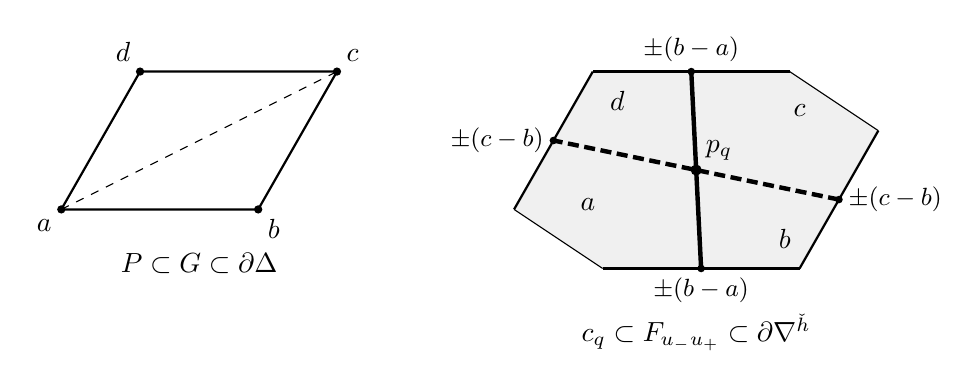
\begin{tikzpicture}[scale=1.25,>=stealth]
\coordinate (a) at (0,0); \coordinate (b) at (2,0); \coordinate (c) at (2.8,1.4); \coordinate (d) at (0.8,1.4);
\draw[thick] (a)--(b)--(c)--(d)--cycle;
\draw[dashed] (a)--(c);
\foreach \p/\l/\pos in {a/a/below left,b/b/below right,c/c/above right,d/d/above left}{\fill (\p) circle (1.2pt); \node[\pos] at (\p) {$\l$};}
\node at (1.4,-0.55) {$P\subset G\subset\partial\Delta$};
\begin{scope}[xshift=4.6cm]
\coordinate (A) at (0,0); \coordinate (As) at (0.9,-0.6); \coordinate (Bs) at (2.9,-0.6);
\coordinate (Cs) at (3.7,0.8); \coordinate (C) at (2.8,1.4); \coordinate (D) at (0.8,1.4);
\fill[gray!12] (A)--(As)--(Bs)--(Cs)--(C)--(D)--cycle;
\draw (A)--(As); \draw (Cs)--(C);
\draw[thick] (As)--(Bs); \draw[thick] (Bs)--(Cs); \draw[thick] (C)--(D); \draw[thick] (D)--(A);
\coordinate (p) at (1.85,0.4);
\coordinate (mab) at (1.9,-0.6); \coordinate (mbc) at (3.3,0.1); \coordinate (mcd) at (1.8,1.4); \coordinate (mda) at (0.4,0.7);
\draw[line width=1.6pt] (mab)--(p)--(mcd);
\draw[line width=1.6pt,dash pattern=on 4pt off 2pt] (mbc)--(p)--(mda);
\foreach \m in {mab,mbc,mcd,mda}{\fill (\m) circle (1.1pt);}
\fill (p) circle (1.6pt); \node[above right] at (p) {$p_q$};
\node at (0.75,0.05) {$a$}; \node at (2.75,-0.3) {$b$}; \node at (2.9,1.0) {$c$}; \node at (1.05,1.1) {$d$};
\node[below] at (mab) {\small $\pm(b-a)$}; \node[above] at (mcd) {\small $\pm(b-a)$};
\node[right] at (mbc) {\small $\pm(c-b)$}; \node[left] at (mda) {\small $\pm(c-b)$};
\node at (1.85,-1.25) {$\mathfrak c_q\subset F_{u_-u_+}\subset\partial\nabla^{\check h}$};
\end{scope}
\end{tikzpicture}
\caption{Left: a node parallelogram $P=abcd$ in a two-face $G$ of $\Delta$, with the diagonal $\{a,c\}$ dashed. Right: its carrying
cell $\mathfrak c_q=P+\operatorname{conv}\tau$ in the two-face $F_{u_-u_+}$ of $\nabla^{\check h}$, drawn for $\tau$ a segment; the
maximal cells $C_\pm$ lie on the two sides of the page. The thick edges have the two-point lower supports $\{a,b\}$, $\{b,c\}$,
$\{c,d\}$, $\{d,a\}$, and the four legs of $\Gamma$ join $p_q$ to their barycentres, labelled with their vanishing vectors. The four
complementary regions carry the charts of the lower rays $a,b,c,d$. The $b-a$ passage (solid) and the $c-b$ passage (dashed) are
the two pairs of opposite legs.}
\label{fig:node}
\end{figure}

\begin{lemma}[the node germ]\label{lem:nodegerm}
\begin{enumerate}
\item For $n\in P$ let $\pi_n$ be the chart $N_\R\to N_\R/\R n$, identified with $H_0=u_+^\perp$ by $x\mapsto x+\langle u_+,x\rangle n$.
Then for $n,n'\in P$,
\[
\pi_{n'}-\pi_n=\begin{cases}-\check h_+\,(n'-n)&\text{on }C_+,\\ -\bigl(\check h_++y_2(x)\bigr)(n'-n)&\text{on }C_-,\end{cases}\qquad
y_2(x):=\alpha(\mathfrak c)-\alpha(x),
\]
and $y_2\ge0$ on $C_+$, $y_2\le0$ on $C_-$, $y_2=0$ on $\mathfrak c$.
\item The affine structure off the discriminant near $\mathfrak c$ is unchanged if $\Gamma\cap\mathfrak c$ is replaced by any
four-legged star in $\mathfrak c$ whose legs end at the barycentres of the four edges of $\mathfrak c$ with a two-point lower
support, the region between consecutive legs receiving the chart of the lower ray of the boundary arc of $\mathfrak c$ that it
contains.
\item Let $b'$ be the centre of a translate $P+z\subset\mathfrak c$, $z$ a vertex of $\operatorname{conv}\tau$, and let
$\Gamma_{b'}$ be a star with vertex $b'$ whose legs leave $b'$ in the directions $\pm(b-a)$, $\pm(d-a)$ and continue inside
$\mathfrak c$ to the barycentres of the edges with lower supports $\{a,d\},\{b,c\},\{a,b\},\{c,d\}$, coinciding with the legs of
$\Gamma$ near these barycentres. Then a neighbourhood of $b'$ is integral affine isomorphic, with integral translations, to a
neighbourhood of the vertex of the discriminant in \cite[Ex.~6.1]{CBM}.
\end{enumerate}
\end{lemma}

\begin{proof}
(1) Since $\langle u_+,n\rangle=-1$, $N=(H_0\cap N)\oplus\Z n$, and $x\mapsto x+\langle u_+,x\rangle n$ is the lattice projection
along $n$ onto $H_0$. Hence $\pi_{n'}-\pi_n=\langle u_+,x\rangle(n'-n)$. On $C_+$, $\langle u_+,x\rangle=-\check h_+$. On $C_-$,
$\langle u_+,x\rangle=\alpha(x)+\langle u_-,x\rangle=\alpha(x)-\check h_-=-\check h_+-y_2(x)$. Since $\nabla^{\check h}$ is convex,
$\langle u_-,x\rangle\ge-\check h_-$ on $C_+$ and $\langle u_+,x\rangle\ge-\check h_+$ on $C_-$, which give the signs of $y_2$.

(2) By (1) the charts $\pi_n$, $n\in P$, differ by integral translations on $C_+$ and on $C_-$ separately, and by a map that is
not affine across $\mathfrak c$. So inside $\mathfrak c$ one needs only a closed set separating four regions, each containing the
vertices of $\mathfrak c$ with a given lower ray. Edges of $\mathfrak c$ with a one-point lower support join vertices with the same
lower ray, and the four edges with a two-point lower support separate the boundary of $\mathfrak c$ into four arcs with lower rays
$a,b,c,d$ in this cyclic order.

(3) Choose the origin at the lattice point $a+z$ and the basis $v_1=b-a$, $w_{u_-}$, $v_3=d-a$ of $H_0\cap N$, where $w_{u_-}$ is the
vector of Lemma~\ref{lem:primheight} for $(u,u')=(u_+,u_-)$: by that lemma $H_0\cap N=N_G\oplus\Z w_{u_-}$, and $v_1,v_3$ is a basis of
$N_G$ because $P$ is a unit parallelogram. Then $\alpha(v_1)=\alpha(v_3)=0$ and $\alpha(w_{u_-})=-1$, so the second coordinate of a point of $H_0$ is
$y_2$. In the coordinates $y=(y_1,y_2,y_3)$ of this basis, the chart of
the corner $a+iv_1+jv_3$ ($i,j\in\{0,1\}$) is, up to an integral translation, $y$ on $\{y_2\ge0\}$ and
$\bigl(I-(ie_1+je_3)e_2^{\mathsf T}\bigr)y$ on $\{y_2\le0\}$, by (1). Near $b'=(\tfrac12,0,\tfrac12)$ the region of the corner
$(i,j)$ is the quadrant $\{\operatorname{sign}(y_1-\tfrac12)=2i-1,\ \operatorname{sign}(y_3-\tfrac12)=2j-1\}$. This is the
atlas of \cite[Ex.~6.1]{CBM}: two triangular prisms glued along a unit square, with perpendicular prism directions $e_1,e_3$, the
monodromy-invariant plane $\langle e_1,e_3\rangle$, and the vertex at the barycentre of the square; the translations are
integral.
\end{proof}

The sign of the shear in (3), forced by the convexity of $\nabla^{\check h}$ through (1), is the one of \cite[Ex.~6.1]{CBM}, where it
is forced by the two prisms. With the barycentric placement, the vertex of $\Gamma$ sits at the barycentre of $\mathfrak c$, whose
position modulo the lattice is in general not that of $b'$; this is why the vertex is moved in (3).

\begin{lemma}[placement]\label{lem:placement}
Let $\Gamma'$ be $\Gamma$ with the star inside every carrying cell replaced by $\Gamma_{b'}$. There is a piecewise linear
homeomorphism $\phi_{\rm pl}$ of $B$ which preserves every closed face of $\nabla^{\check h}$ and every cell of $\mathscr P$, carries
$\Gamma'$ onto $\Gamma$ and the local system of $B\setminus\Gamma'$ to that of $B\setminus\Gamma$, and is supported in a compact
subset of the union of the open stars of the points $p_q$ in $\operatorname{Bar}\mathscr P$. It is isotopic to the identity
through homeomorphisms with the same support that preserve $\Gamma$ outside the carrying cells.
\end{lemma}

\begin{proof}
Both stars lie in the disc $\mathfrak c$, have the same four end points on $\partial\mathfrak c$, coincide near them, and have their
legs in the same cyclic order. So there is a piecewise linear homeomorphism of $\mathfrak c$, equal to the identity near
$\partial\mathfrak c$, carrying one to the other; by the Alexander trick \cite{Ale23}, \cite[Lemma~2.1]{FM12} it is isotopic to the
identity relative to a neighbourhood of $\partial\mathfrak c$. Extend it and the isotopy across the two sides of $\mathfrak c$ by a
product in a thin collar, tapering to the identity. The support is then a compact subset of the open star of $p_q$, which is an
open neighbourhood of $\operatorname{int}\mathfrak c$. By Lemma~\ref{lem:nodegerm}(2) both placements assign the charts to the four
complementary regions by the same rule, and $\phi_{\rm pl}$ preserves the regions, so it carries $\Lambda$ to $\Lambda$.
\end{proof}

The open stars of distinct points $p_q$ in $\operatorname{Bar}\mathscr P$ are disjoint, because no chain of cells contains two
different two-cells; so the modifications at different nodes do not interact. This holds even when the closed carrying cells of
two nodes meet, which happens: at an $A_1$ hexagon they may share a vertex with lower ray $o$, at a pentagon or an $A_2$ hexagon
they may share an edge with lower support $\{o,w\}$, and across an edge of $\Delta$ they may share an edge whose barycentre is a positive
vertex of $\Gamma$.

\begin{proof}[Proof of Proposition~\ref{prop:base}(2)]
The germ is described by Lemma~\ref{lem:nodegerm}(3), and the comparison of the two placements is
Lemma~\ref{lem:placement}.
\end{proof}

We work with the barycentric placement from now on; the node point is $p_q=b_{\mathfrak c_q}$. Relative tropical $2$-cycles
(Definition~\ref{def:relcycle}) are defined on triangulations in which $\Gamma$ is full, and $\operatorname{Bar}\mathscr P$ is
one by Lemma~\ref{lem:full}.


The stalks of $\iota_*\Lambda$ at the points of $\Gamma$ are computed in Lemma~\ref{lem:stalks}: on a leg in $F_{uu'}$, at a
negative vertex and at a node point of $F_{uu'}$ the stalk is $\{u,u'\}^\perp\cap N$, and at a positive vertex on the edge of
$\nabla^{\check h}$ dual to the triangle $\{u_1,u_2,u_3\}$ it is $\{u_1,u_2,u_3\}^\perp\cap N=\Z d$, with $d$ the common vanishing vector of
the three legs.

\emph{The discriminant in a two-face.} Let $G$ be a pentagon or a hexagon, $G^\circ=[u_-,u_+]$. Each node parallelogram $P$ of
$\sigma|_G$ has two legs whose lower supports are interior edges $[o,w]$ of $\sigma|_G$, which share the lower ray $o$ and are therefore
adjacent in the cyclic order at $p_q$, and two legs whose lower supports are edges of $\Delta$.

\begin{lemma}[arcs across interior edges]\label{lem:dualarc}
Let $\epsilon=[o,w]$ be an interior edge of $\sigma|_G$, and let $L$ and $L'$ be the two cells of $\sigma|_G$ containing it, with
two-cells $\mathfrak c_L$, $\mathfrak c_{L'}\subset F_{u_-u_+}$ as above. Then $\Gamma$ contains an arc from $b_{\mathfrak c_L}$ to
$b_{\mathfrak c_{L'}}$ that is a union of legs with lower support $\{o,w\}$, vanishing vector $\pm(w-o)$ and covector $\pm(u_+-u_-)$,
and whose interior points are edge points of $\Gamma$.
\end{lemma}

\begin{proof}
Let $\Gamma_\epsilon$ be the union of the legs with lower support $\{o,w\}$, a subgraph of $\Gamma$. The facet indices of the maximal cells
at such a leg take the value $-1$ at $o$, so they are $u_-$ and $u_+$, the only lattice points of $\Delta^\circ$ with this property ($o$ is
interior to $G$, and $G^\circ\cap M=\{u_-,u_+\}$). So every such leg lies in a two-cell $f\subset F_{u_-u_+}$ whose lower support contains
$\epsilon$: the segment $\epsilon$ itself, or a two-cell of $\Sigma'$ containing $\epsilon$ on which $u_\pm$ take the value $-1$, that is, $L$
or $L'$. We compute the number of legs of $\Gamma_\epsilon$ at each point.
\begin{itemize}
\item At $b_e$, $e$ an edge with lower support $\epsilon$: the facet indices around $e$ lie in $\{u_-,u_+\}$. If $e$ lies in one facet, so
that $j=1$ in Lemma~\ref{lem:edge}, no leg ends at $b_e$. If $b_e\in\Gamma_\epsilon$, then $j=2$, and by Lemma~\ref{lem:edge} exactly two legs
end at $b_e$, both with the lower support of $e$.
\item At $b_f$, $f$ a two-cell with lower support $\epsilon$ and $u_+(f)\ne u_-(f)$: $f$ has exactly two edges with lower support $\epsilon$
and no other edge with a two-point lower support, so two legs of $\Gamma_\epsilon$ end at $b_f$.
\item At $b_{\mathfrak c_L}$: the unique edge of $\mathfrak c_L$ with lower support $\epsilon$, the face selected by the outer normal of
$\epsilon$ in $L$, gives exactly one leg of $\Gamma_\epsilon$; likewise at $b_{\mathfrak c_{L'}}$. By the stack lemma no other two-cell over
$L$ or $L'$ carries a leg.
\end{itemize}
So $\Gamma_\epsilon$ is a finite graph in which $b_{\mathfrak c_L}$ and $b_{\mathfrak c_{L'}}$ have valency one and every other vertex has
valency two. The component of $b_{\mathfrak c_L}$ is therefore a path, whose other end has valency one and is not $b_{\mathfrak c_L}$; it is
$b_{\mathfrak c_{L'}}$. Its interior points are points $b_e$ in the interior of $F_{u_-u_+}$ and points $b_f$ with a two-point lower
support, which are edge points by Lemma~\ref{lem:types}. All its legs have the vanishing vector $\pm(w-o)$ and the covector $\pm(u_+-u_-)$.
\end{proof}

By Proposition~\ref{prop:L2}(2) this arc is the only arc of $\Gamma$ with lower support $\{o,w\}$. Applied to the interior edges
of Lemma~\ref{lem:subdiv}(3), the lemma gives the shape of $\Gamma$ in the two-face $F_{u_-u_+}$ of a del Pezzo face: at a pentagon, a cycle
through the two nodes and the negative vertex of the triangle, with one arc from node to node (across $[o,w_1]$ in the
coordinates~\eqref{eq:pentnormal}); at an $A_1$ hexagon, a cycle through the two nodes and the two negative vertices, with no arc from node
to node; at an $A_2$ hexagon, three arcs from node to node, across the edges $[o,w_j]$ with $j\equiv j_0\bmod2$, forming a cycle of
$\Gamma$ through the three nodes with no trivalent vertex. These configurations are used in Section~\ref{sec:cycles}; the lift of
Section~\ref{sec:lift} treats several nodes in one two-face in Section~\ref{ssec:lift-assembly}, and the resolution side in
Lemma~\ref{lem:resmove}.

\subsection{The mirror subdivision}\label{ssec:mirrorsub}
The mirror family of Section~\ref{ssec:mirrorfamily} uses a height $H=k_0\varphi+h_C$ on $\partial\Delta\cap N$, where $h_C$ induces a
refinement $\mathcal F_C$ of $\Sigma'$. The analysis near the node points (Section~\ref{ssec:member}) needs two properties of
$\mathcal F_C$: it agrees with $\Sigma'$ on the faces of dimension at most two, so that every node parallelogram is a cell, and the
three-cells of $\mathcal F_C$ containing a node parallelogram $P$ have all their lattice points off $P$ at lattice height one over the
plane of $P$. We construct $\mathcal F_C$ by pulling the lattice points of $\partial\Delta$ that are not vertices of $\Sigma'$, and show that
the second property then holds automatically. The subdivision $\Sigma'$ itself need not have it (Remark~\ref{rem:Sigmaheight}).

\emph{Fans and subdivisions of $\mathcal A$.} Let $\mathcal A=(\partial\Delta\cap N)\cup\{0\}$. We use the language of point configurations
\cite{DLRS}. A subdivision $\mathcal S$ of $\mathcal A$ is \emph{regular} if it is induced by a height $g\colon\mathcal A\to\R$: its cells are
the subsets $\mathfrak d=\{a\in\mathcal A:g(a)=\ell_{\mathfrak d}(a)\}$ for the affine functions $\ell_{\mathfrak d}\le g$ on $\mathcal A$ whose
equality set spans a face of the lower hull. Let $\hat g\colon\operatorname{conv}\mathcal A\to\R$ be the lower envelope, the largest convex
function with $\hat g\le g$ on $\mathcal A$; then $\hat g=\ell_{\mathfrak d}$ on $\operatorname{conv}\mathfrak d$, and
$\{\hat g=\ell_{\mathfrak d}\}=\operatorname{conv}\mathfrak d$. A complete fan in $N_\R$ that refines the fan over the faces of $\Delta$ and has
its rays generated by points of $\mathcal A$ is the fan of cones from $0$ over the cells of a subdivision of $\mathcal A$ all of whose maximal
cells contain $0$, the cells on $\partial\Delta$ being those of the fan; the fan carries a strictly convex piecewise linear function if and
only if the subdivision is regular, the function, normalised to vanish at $0$, being a height that induces the subdivision. By~\ref{hyp:P},
$\Sigma'$ is regular in this sense. A point $j\in\mathcal A$ is a \emph{vertex} of $\mathcal S$ if $\{j\}$ is a cell.

\begin{definition}[pulling]\label{def:pulling}
Let $\mathcal S$ be a subdivision of $\mathcal A$ and $j\in\mathcal A$. The \emph{pulling} $\operatorname{pull}_j\mathcal S$ keeps every cell
$\mathfrak d$ with $j\notin\operatorname{conv}\mathfrak d$, and replaces every cell $\mathfrak d$ with $j\in\operatorname{conv}\mathfrak d$ by the
cells $\{j\}\cup(\mathfrak d\cap F)$, for the faces $F$ of $\operatorname{conv}\mathfrak d$ with $j\notin F$ \cite[\S4.3]{DLRS}.
\end{definition}

The definition applies to every cell whose convex hull contains $j$, also when $j$ is not a point of the cell, as happens after an
earlier pulling has placed $j$ strictly above the lower hull.

\begin{lemma}[pulling preserves regularity]\label{lem:pullreg}
Let $g$ induce $\mathcal S$ and let $j\in\mathcal A$. Put $g_\eta(j)=\hat g(j)-\eta$ and $g_\eta=g$ on $\mathcal A\setminus\{j\}$. For $\eta>0$ small,
$g_\eta$ induces $\operatorname{pull}_j\mathcal S$. In particular $\operatorname{pull}_j\mathcal S$ is regular, $j$ is one of its vertices, and every
vertex of $\mathcal S$ other than $j$ remains a vertex. If $j\in\partial\Delta$ and every maximal cell of $\mathcal S$ contains $0$, then every
maximal cell of $\operatorname{pull}_j\mathcal S$ contains $0$.
\end{lemma}

\begin{proof}
Let $\mathfrak d$ be a cell with $j\in\operatorname{conv}\mathfrak d$, and $F$ a facet of $\operatorname{conv}\mathfrak d$ with $j\notin F$. Let
$\lambda_F$ be the affine function on $\operatorname{aff}\mathfrak d$, extended to the ambient space, with $\lambda_F=0$ on $F$ and $\lambda_F(j)=1$;
it is positive on $\operatorname{conv}\mathfrak d\setminus F$. The affine function $\ell_{\mathfrak d}-\eta\lambda_F$ agrees with $g_\eta$ at $j$,
because $\ell_{\mathfrak d}(j)=\hat g(j)$, and on $\mathfrak d\cap F$; it lies strictly below $g_\eta=g=\ell_{\mathfrak d}$ on
$\mathfrak d\setminus(F\cup\{j\})$. At a point $a\in\mathcal A\setminus(\mathfrak d\cup\{j\})$ we have $g(a)>\ell_{\mathfrak d}(a)$, and since $\mathcal A$ is
finite, $\ell_{\mathfrak d}(a)-\eta\lambda_F(a)<g(a)$ for $\eta$ small. So $\{j\}\cup(\mathfrak d\cap F)$ is a cell of the subdivision induced by
$g_\eta$, with convex hull $\operatorname{conv}(\{j\}\cup F)$; these convex hulls, over the facets $F$ not containing $j$, cover
$\operatorname{conv}\mathfrak d$. If $j\notin\operatorname{conv}\mathfrak d$, then $\hat g(j)>\ell_{\mathfrak d}(j)$, because
$\{\hat g=\ell_{\mathfrak d}\}=\operatorname{conv}\mathfrak d$; so for $\eta$ small $\ell_{\mathfrak d}(j)<g_\eta(j)$, and $\mathfrak d$ remains a
cell. Applying this to the maximal cells, the cells found cover $\operatorname{conv}\mathcal A$, so they are all the maximal cells of the
subdivision induced by $g_\eta$, which is therefore $\operatorname{pull}_j\mathcal S$. The point $j$ is a vertex of every cell
$\operatorname{conv}(\{j\}\cup F)$, and a vertex $v\ne j$ of $\mathcal S$ is kept because $j\notin\operatorname{conv}\{v\}$.

For the last statement, a maximal cell of $\mathcal S$ with $j$ in its convex hull is $\operatorname{conv}(\{0\}\cup C)$ with $C$ a cell on
$\partial\Delta$, and $j\in\operatorname{conv}C$ because $j\in\partial\Delta$ and $C$ lies in a supporting hyperplane of $\Delta$. The facets of
$\operatorname{conv}(\{0\}\cup C)$ are $C$ and the cones $\operatorname{conv}(\{0\}\cup F')$ over the facets $F'$ of $C$; those not containing
$j$ are of the second kind and contain $0$.
\end{proof}

Let $\mathcal F_C$ be the subdivision of $\partial\Delta$ obtained from $\Sigma'$ by pulling, one at a time and in any order, the lattice points
of $\partial\Delta$ that are not vertices of $\Sigma'$. By Lemma~\ref{lem:pullreg} it is induced by a height on $\mathcal A$, which we may take
rational; the function on $N_\R$ that is linear on the cone over each cell and equal to this height on its vertices is strictly convex on the
fan over $\mathcal F_C$. Multiplying it by a positive integer makes its linear functions integral. We let $h_C$ be such a function: strictly
convex on the fan over $\mathcal F_C$, inducing $\mathcal F_C$, with integral slopes and $h_C(0)=0$.

\begin{lemma}[the pyramid over a unit parallelogram]\label{lem:pyramid}
Let $P=abcd\subset G$ be a node parallelogram, $G^\circ=[u,u']$, and let $x\in u^\vee\cap N$ with $h_x:=e_{u'}(x)\ge1$. With $w_{u'}$ as in
Lemma~\ref{lem:primheight}, write
\[
x-a=\alpha(b-a)+\beta(d-a)+h_x\,w_{u'},\qquad\alpha,\beta\in\Z.
\]
Then $y:=a+\lceil\alpha/h_x\rceil(b-a)+\lceil\beta/h_x\rceil(d-a)+w_{u'}$ is the only lattice point of $\operatorname{conv}(P\cup\{x\})$ with
$e_{u'}=1$. If $h_x\ge2$, then $y$ is not a vertex of $\operatorname{conv}(P\cup\{x\})$.
\end{lemma}

\begin{proof}
By Lemma~\ref{lem:primheight}, $(b-a,d-a,w_{u'})$ is a basis of $u^\perp\cap N$, since $b-a,d-a$ is a basis of $N_G$ ($P$ is a unit parallelogram).
In the lattice coordinates $(s,t,e)$ of this basis with origin $a$ on $\operatorname{aff}(u^\vee)$, $e=e_{u'}$, $P=[0,1]^2\times\{0\}$ and
$x=(\alpha,\beta,h_x)$. The slice of $\operatorname{conv}(P\cup\{x\})$ at $e=1$ is $(1-1/h_x)P+x/h_x$, the product of the intervals
$[\alpha/h_x,\alpha/h_x+1-1/h_x]$ and $[\beta/h_x,\beta/h_x+1-1/h_x]$. Each has length $1-1/h_x$ and end points in $\frac1{h_x}\Z$; writing
$\alpha=mh_x+i$ with $0\le i<h_x$, the first interval is $[m+i/h_x,\,m+(i+h_x-1)/h_x]$, which contains exactly one integer, $\lceil\alpha/h_x\rceil$;
likewise for $\beta$. The vertices of $\operatorname{conv}(P\cup\{x\})$ lie at the levels $0$ and $h_x$, so for $h_x\ge2$ the point $y$ at level $1$ is
not a vertex.
\end{proof}

\begin{lemma}[a high apex forces a lattice point]\label{lem:hidden}
Let $\mathcal S$ be a subdivision of $\partial\Delta$ into lattice polytopes that induces $\sigma$ on the two-faces of $\Delta$. Let $P\subset G$ be a
node parallelogram, $G^\circ=[u,u']$, and $\omega$ the three-cell of $\mathcal S$ in $u^\vee$ containing $P$. If some vertex $x$ of $\omega$ has
$e_{u'}(x)\ge2$, then the point $y$ of Lemma~\ref{lem:pyramid} is a lattice point of $\omega$ that is not a vertex of $\omega$, and it lies in the
relative interior of the facet $u^\vee$.
\end{lemma}

\begin{proof}
$y\in\operatorname{conv}(P\cup\{x\})\subseteq\omega$. A vertex of $\omega$ lying in the subpolytope $\operatorname{conv}(P\cup\{x\})$ is a vertex of it,
and by Lemma~\ref{lem:pyramid} $y$ is not. Suppose $y$ lay in a face $G''$ of $\Delta$ of dimension at most two; we may take $G''\subseteq u^\vee$.
Then $\omega\cap G''$ is a face of $\omega$, hence a cell of $\mathcal S$ contained in $G''$, that is, a cell of $\sigma$ or a face of one. Such a cell
has no lattice points other than its vertices (Lemma~\ref{lem:subdiv}(4)), so $y$ would be a vertex of $\omega\cap G''$, hence of $\omega$, a
contradiction.
\end{proof}

\begin{proposition}\label{prop:pulling}
Let $\Delta$ be admissible and $\sigma$ a profile satisfying~\ref{hyp:P}, with any number of pentagons and of hexagons on either
branch. Then:
\begin{enumerate}
\item $\mathcal F_C$ is regular: there is a function $h_C$ with integral slopes, strictly convex on the fan over $\mathcal F_C$, that induces
$\mathcal F_C$; every maximal cell of the corresponding subdivision of $\mathcal A$ contains $0$;
\item $\mathcal F_C$ refines $\Sigma'$ and agrees with it on the faces of $\Delta$ of dimension at most two; so the two-cells of $\mathcal F_C$ in
two-faces of $\Delta$ are unimodular triangles and node parallelograms;
\item every lattice point of $\partial\Delta$ is a vertex of $\mathcal F_C$;
\item \emph{(height condition)} for every node parallelogram $P\subset G$, $G^\circ=[u,u']$, let $\omega_1\subseteq u^\vee$ and
$\omega_2\subseteq u'^\vee$ be the three-cells of $\mathcal F_C$ containing $P$. Every lattice point of $\omega_1$ not in $P$ has $e_{u'}=1$, and
every lattice point of $\omega_2$ not in $P$ has $e_u=1$.
\end{enumerate}
\end{proposition}

\begin{proof}
(1) By Lemma~\ref{lem:pullreg}, applied at each step, $\mathcal F_C$ is induced by a height on $\mathcal A$ and every maximal cell of
the corresponding subdivision of $\mathcal A$ contains $0$; the integral slopes of $h_C$ come from the choice of $h_C$ after the
definition of $\mathcal F_C$. (2) Pulling $j$ changes only the cells whose convex hull contains $j$, and refines
them. Every lattice point of a face of dimension at most two lies in $R$ and is a vertex of $\Sigma'$ (Section~\ref{ssec:faces}), so every
pulled point lies in the relative interior of a facet of $\Delta$, and no cell in a face of dimension at most two contains it. By induction
these cells are never changed. (3) Each pulled point becomes a vertex, and vertices are never lost (Lemma~\ref{lem:pullreg}).

(4) Let $\omega=\omega_1$. The set $\omega\cap u'^\vee=\omega\cap G$ is a face of $\omega$ and, by (2), a cell of $\sigma$ in $G$ containing $P$; so it is
$P$. Hence every vertex of $\omega$ off $P$ has $e_{u'}\ge1$. If a vertex had $e_{u'}\ge2$, Lemma~\ref{lem:hidden} would give a lattice point of
$\omega$ that is not a vertex of $\omega$; by (3) it is a vertex of $\mathcal F_C$, and a vertex of a polyhedral complex that lies in a cell is a
vertex of that cell. So every vertex of $\omega$ off $P$ has $e_{u'}=1$. As $e_{u'}$ is affine and takes values in $[0,1]$ on $\omega$, every lattice
point of $\omega$ has $e_{u'}\in\{0,1\}$, and those with $e_{u'}=0$ lie in $\omega\cap G=P$. The statement for $\omega_2$ follows by exchanging $u$
and $u'$.

The face type enters only through three facts, which hold for every profile: $\ell(G^\circ)=1$ at the face of $P$ (used in
Lemma~\ref{lem:primheight}); every cell of $\sigma$, and every face of one, has no lattice points besides its vertices (used in
Lemma~\ref{lem:hidden}; Lemma~\ref{lem:subdiv}(4) for pentagons and for hexagons on both branches); and every point of $R$, the hexagon centres
included, is a vertex of $\Sigma'$ (used in (2)). A node parallelogram is a two-cell of $\sigma|_G$, so no other cell of $\sigma|_G$ contains it; at an
$A_2$ hexagon this applies to each of the three rhombi, although they share edges pairwise.
\end{proof}

The lattice points of $\omega_1\cup\omega_2$ not in $P$ are the \emph{apexes} of $P$ in Section~\ref{ssec:member}. The proof of (4) shows more.

\begin{remark}\label{rem:Sigmaheight}
\begin{enumerate}
\item Let $\mathcal S$ be a regular subdivision of $\partial\Delta$ into lattice polytopes that induces $\sigma$ on the two-faces and in which the
three-cells containing node parallelograms have no lattice points other than their vertices. Then the height condition holds for $\mathcal S$, by
the argument of (4) with Lemma~\ref{lem:hidden}. In particular it holds for $\Sigma'$ itself whenever every lattice point of $\partial\Delta$ is a
vertex of $\Sigma'$; this is the case for the subdivisions $\Sigma'$ of the examples $X_9$, $X_{19}$ and $X_{20}$ in Section~\ref{sec:examples}, and there
$\mathcal F_C=\Sigma'$.
\item In general a subdivision $\Sigma'$ satisfying~\ref{hyp:P} does not satisfy the height condition. The polytope $\Delta_9$ of the example
$X_9$ has a subdivision satisfying~\ref{hyp:P} whose vertices are all the lattice points of $\partial\Delta_9$ except $(-1,0,0,0)$; in it the three-cell over one of the pentagon parallelograms $P$, in the facet $u=(1,-1,-1,-1)$ with
$u'=(0,1,-1,-1)$, is the pyramid $\operatorname{conv}(P\cup\{(0,1,0,0)\})$ with $e_{u'}((0,1,0,0))=2$, whose only lattice point at height one is $(-1,0,0,0)$.
Pulling this point gives the $\Sigma'$ of Section~\ref{sec:examples}. On the list of Section~\ref{ssec:list}, the subdivisions $\Sigma'$ that
the linear program of~\ref{hyp:P} returns violate the height condition on $7$ of the $364$ hexagon-free polytopes satisfying~\ref{hyp:P}, with apexes
at height $2$ or $3$, while $\mathcal F_C$ satisfies it on all of them (exact computation).
\end{enumerate}
\end{remark}

\subsection{When (Proj) fails}\label{ssec:proj}
This section does not assume~\ref{hyp:P}. We show that~\ref{hyp:P} is equivalent to the projectivity of $X'_\sigma\to X$, and describe what a failure
means for the exceptional surfaces. For an interior edge $\epsilon=[o,w_j]$ of $\sigma|_G$, $G$ a pentagon or a hexagon, put
\[
I_\epsilon:=e_{w_{j-1}}+e_{w_{j+1}}-a_je_{w_j}+(a_j-2)e_o\in\Z^R,\qquad (w_{j-1}-o)+(w_{j+1}-o)=a_j(w_j-o).
\]
For a function $\psi$ on $G\cap N$ that is affine on the cells $L\supset T_{j-1}$ and $L'\supset T_j$ of $\sigma|_G$ at $\epsilon$,
$\langle I_\epsilon,\psi\rangle=\psi(w_{j+1})-\ell_L(w_{j+1})$, where $\ell_L$ is the affine function equal to $\psi$ on $L$: the \emph{bend} of $\psi$
across $\epsilon$, measured at a point at lattice distance one from $\epsilon$.

\begin{lemma}\label{lem:projLP}
\ref{hyp:P} holds if and only if there is $\psi\in\Q^R$ with $\langle\circv_q,\psi\rangle=0$ for every $q\in Q$ and $\langle I_\epsilon,\psi\rangle>0$ for every
interior edge $\epsilon$ of $\sigma$ at a pentagon or a hexagon.
\end{lemma}

\begin{proof}
A function $\psi$ on $G\cap N$ induces $\sigma|_G$ if and only if it is affine on each cell, which for a parallelogram is $\langle\circv_q,\psi\rangle=0$,
and bends positively across each interior edge; local convexity across the interior edges implies convexity on $G$. If~\ref{hyp:P} holds, the
restriction to $R$ of a strictly convex function inducing $\Sigma'$ has these properties. Conversely, given $\psi$, let $\mathcal S_\Phi$ be the
regular subdivision of $\Phi\cap R$ induced by $\psi$ on each facet $\Phi$ of $\Delta$. On a face of $\Phi$ it restricts to the regular subdivision
induced by the restriction of $\psi$, which on two-faces is $\sigma$ and on edges is trivial; so the $\mathcal S_\Phi$ agree on common faces and form a
subdivision $\mathcal S$ of $\partial\Delta$ with vertices in $R$. Let $g$ be the function on $N_\R$ that is linear on the cone over each cell of
$\mathcal S$ and equals $\psi$ on $R$. It is convex across the walls inside the cones over facets. The function $\varphi$ that equals $1$ on
$\partial\Delta$ and is linear on the cones over the facets is convex, with positive bend across each wall between two facet cones, and linear
inside them; so for $\gamma$ large, $g+\gamma\varphi$ is strictly convex on the fan over $\mathcal S$. The toric variety of this fan is projective, its rays pass
through points of $R\subset\partial\Delta$, and it induces $\sigma$.
\end{proof}

Let $\widehat X$ be the small resolution with the chosen diagonals, which exists as a compact complex manifold without~\ref{hyp:P}
(Section~\ref{ssec:partialres}). For an interior edge $\epsilon=[o,w_j]$ of $\sigma|_G$, let $f_\epsilon\subset E'_G$ be the torus-invariant curve of
the cone over $\epsilon$ in the local model $U'_{G,\sigma}$, and $\tilde f_\epsilon\subset E_G$ its proper transform in $\widehat X$, which is the
curve $f_j$ of Proposition~\ref{prop:classical}. In the local model of $\widehat X$ the curve $\tilde f_\epsilon$ is the curve of the wall
$\operatorname{cone}(o,w_j)$ between the cones over $T_{j-1}$ and $T_j$, and the wall relation
$w_{j-1}+w_{j+1}-a_jw_j+(a_j-2)o=0$ gives $(D_r\cdot\tilde f_\epsilon)_{r\in R}=I_\epsilon$.

\begin{proposition}\label{prop:projective}
The following are equivalent:
\begin{enumerate}
\item \ref{hyp:P} holds;
\item $X'_\sigma\to X$ is projective;
\item there are no rational numbers $y_\epsilon\ge0$, not all zero, and $\nu_q$ with
$\sum_\epsilon y_\epsilon[\tilde f_\epsilon]=\sum_q\nu_q[C_q]$ in $H_2(\widehat X;\Q)$.
\end{enumerate}
\end{proposition}

\begin{proof}
(1)$\Rightarrow$(2): $X'_\sigma\to X$ is induced by the projective morphism $P'_\sigma\to\mathbb P_\Delta$. (2)$\Rightarrow$(3): let $L$ be relatively
ample for $X'_\sigma\to X$ and $\pi\colon\widehat X\to X'_\sigma$. Then $\pi^*L\cdot C_q=0$, since $C_q$ is contracted by $\pi$, and
$\pi^*L\cdot\tilde f_\epsilon=L\cdot f_\epsilon>0$, since $f_\epsilon$ is a curve in a fibre of $X'_\sigma\to X$. A relation as in (3) would pair with
$\pi^*L$ to a positive number on the left and to $0$ on the right. (3)$\Rightarrow$(1): if~\ref{hyp:P} fails, the linear system of
Lemma~\ref{lem:projLP} is infeasible, and by the Farkas--Motzkin alternative there are $y_\epsilon\ge0$, not all zero, and $\nu_q$ with
$\sum_\epsilon y_\epsilon I_\epsilon=\sum_q\nu_q\circv_q$ in $\Q^R$. By Proposition~\ref{prop:partialres}(2) and the computation above, the class
$\sum_\epsilon y_\epsilon[\tilde f_\epsilon]-\sum_q\nu_q[C_q]$ has zero image under~\eqref{eq:injection}, which is injective without~\ref{hyp:P}
(Lemma~\ref{lem:H2}); so it vanishes.
\end{proof}

A relation as in (3) is a \emph{Farkas certificate}. Where~\ref{hyp:P} fails there is no toric variety $P'_\sigma$, no subdivision
$\Sigma'$ and no base $B'_\sigma$, and the methods of this paper do not apply.
